%% —-----------------------------------------------------------
%% sbcreviews-pt.tex
%% Template para SBC Reviews 
%% (https://journals-sol.sbc.org.br/index.php/reviews/) 
%% 
%% Esta versão do template para a SBC Reviews inclui algumas
%% modificações sobre o template original da REIC
%% (https://journals-sol.sbc.org.br/index.php/reic)
%%
%% Licença CC BY 4.0 (https://creativecommons.org/licenses/by/4.0/)
%% Sociedade Brasileira de Computação.

\documentclass[portuguese]{sbcreviews-2025}
\usepackage[misc,geometry]{ifsym} 

%\usepackage{graphicx} % carregada dentro da classe
%\usepackage{fontspec} % carregada dentro da classe
%\usepackage{fontawesome} % carregada dentro da classe
%\usepackage{color} % carregada dentro da classe
%\usepackage{hyperref} % carregada dentro da classe

\usepackage{aas_macros}
\usepackage[bottom]{footmisc}

\usepackage{tabularray}
% O pacote tabularray torna o uso dos pacotes abaixo desnecessarios.
%\usepackage{supertabular}
%\usepackage{multicol}
%\usepackage{multirow}

\usepackage{afterpage}
\usepackage{url}
\usepackage{pifont}

\setcitestyle{round}

\definecolor{engtitle}{rgb}{0.5,0.5,0.5}
\definecolor{orcidlogo}{rgb}{0.37,0.48,0.13}
\definecolor{unilogo}{rgb}{0.16, 0.26, 0.58}
\definecolor{maillogo}{rgb}{0.58, 0.16, 0.26}
\definecolor{darkblue}{rgb}{0.0,0.0,0.0}
\hypersetup{colorlinks,breaklinks,
            linkcolor=darkblue,urlcolor=darkblue,
            anchorcolor=darkblue,citecolor=darkblue}
%\hypersetup{colorlinks,citecolor=blue,linkcolor=blue,urlcolor=blue}
% We disable hyperlinks by default with this line, to avoid the error "\pdfendlink ended up in different nesting level" while writing.

% \jid{ROCS}
% \jtitle{SBC Computing Reviews, 202X, XX:1}
% \issn{}
% \doi{10.5753/rocs.202X.XXXXXX}
% \copyrightstatement{This work is licensed under a Creative Commons Attribution 4.0 International License}
% \jyear{202X}

% \category{Revisão da Literatura}
\title[Template da SBC Reviews 2025 para artigos em português]{Simulação de Arquitetura de Controle para Coordenação de Múltiplos Drones}

% \engtitle{\textcolor{engtitle}{Presenting the SBC Reviews 2025 template - Version for papers in Portuguese}}

%THE ORCID IS MANDATORY FOR EACH AUTHOR
\author[Alencar et al. 2025]{

\affil{\textbf{Jadsonlee da Silva Sá}~\orcidlink{0009-0009-2637-5998}~\textcolor{blue}{\faEnvelope}~~[{Universidade Federal do Vale do São Francisco}~|\href{mailto: jadsonlee.sa@univasf.edu.br}{~{\textit{jadsonlee.sa@univasf.edu.br}}}~]}

\affil{\textbf{Rosalvo Ferreira de Oliveira Neto}~\orcidlink{0009-0009-2637-5998}~\textcolor{blue}{\faEnvelope}~~[{Universidade Federal do Vale do São Francisco}~|\href{mailto: rosalvo.oliveira@univasf.edu.br}{~{\textit{rosalvo.oliveira@univasf.edu.br}}}~]}

\affil{\textbf{Daniel Alencar Penha Carvalho}~\orcidlink{0009-0009-2637-5998}~\textcolor{blue}{\faEnvelope}~~[{Universidade Federal do Vale do São Francisco}~|\href{mailto: daniel.apcarvalho@discente.univasf.edu.br}{~{\textit{daniel.apcarvalho@discente.univasf.edu.br}}}~]}

}

\begin{document}

\begin{frontmatter}

\maketitle

\begin{mail}
Universidade Federal do Vale do São Francisco, Av. Antônio C. Magalhães, 510 - Santo Antonio, Juazeiro, Bahia, 48902-300, Brasil. 
\end{mail}


\begin{abstract-pt}
O uso de drones em missões cooperativas tem ganhado destaque em aplicações como monitoramento ambiental, logística e operações de resgate. Este trabalho investiga estratégias de controle capazes de coordenar grupos de drones em diferentes cenários, analisando formações, dinâmicas de voo e requisitos de cooperação entre veículos. O estudo contempla a modelagem matemática das abordagens selecionadas, bem como sua implementação prática utilizando Python, o protocolo MAVLink e o ecossistema PX4/ArduPilot, além da validação por meio de simulações em ambientes como o Gazebo. O objetivo é definir uma arquitetura de sistema que permita a coordenação autônoma, eficiente e adaptável de múltiplos drones. Como contribuição, este trabalho apresenta uma estrutura flexível para o controle cooperativo de frotas, com potencial aplicação em sistemas autônomos reais.

\end{abstract-pt}

\begin{abstract-en}
The use of drones in cooperative missions has gained prominence in applications such as environmental monitoring, logistics, and rescue operations. This work investigates control strategies capable of coordinating groups of drones in different scenarios, analyzing formations, flight dynamics, and cooperation requirements among the vehicles. The study includes the mathematical modeling of the selected approaches, as well as their practical implementation using Python, the MAVLink protocol, and the PX4/ArduPilot ecosystem, in addition to validation through simulations in environments such as Gazebo. The objective is to define a system architecture that enables autonomous, efficient, and adaptable coordination of multiple drones. As a contribution, this work presents a flexible framework for cooperative fleet control, with potential applications in real-world autonomous systems.
\end{abstract-en}

\begin{pchaves}
Controle de múltiplos drones, Coordenação de drones, Drones cooperativos, Inteligência de enxame, MAVLink
\end{pchaves}

\begin{keywords}
Multi-drone control, Drone coordination, Cooperative drones, Swarm intelligence, MAVLink
\end{keywords}

% \begin{dates}
% This information will be provided by the editor before publishing the paper
% \noindent{\sffamily\textbf{Recebido/Received:}} DD Month YYYY~~~$\bullet$~~~
% {\sffamily\textbf{Aceito/Accepted:}} DD Month YYYY~~~$\bullet$~~~
% {\sffamily\textbf{Publicado/Published:}} DD Month YYYY
% \end{dates}


% \begin{license}
% Published under the Creative Commons Attribution 4.0 International Public License (CC BY 4.0)
% \end{license}

\end{frontmatter}


\section{Introdução}
\label{sec:intro}

O desenvolvimento de Veículos Aéreos Não Tripulados (VANTs) ou do termo em inglês, Unmanned Aerial Vehicles (UAVs), popularmente conhecidos como \textit{drones}, tem crescido exponencialmente nas últimas décadas, impulsionado pelo avanço em áreas como eletrônica embarcada, sensores, comunicação sem fio e algoritmos de controle. Inicialmente restritos a aplicações militares, os VANTs tornaram-se elementos fundamentais em um vasto conjunto de contextos civis e científicos, como monitoramento ambiental, mapeamento geográfico, inspeções industriais, agricultura de precisão e resposta a desastres \citep{chung2018survey, hong2020swarm}. Essa expansão foi acompanhada por um aumento da autonomia e da capacidade de processamento dos sistemas embarcados, permitindo o surgimento de arquiteturas de controle mais sofisticadas e cooperativas.

Entretanto, apesar dos avanços, a operação isolada de um único VANT apresenta limitações inerentes, especialmente em termos de cobertura espacial, redundância e tolerância a falhas. Essas restrições motivaram a transição para abordagens cooperativas envolvendo múltiplos veículos, conhecidas como \textit{enxames de VANTs} (\textit{UAV swarms}) \citep{bu2024advancement}. Nesses sistemas, diversos VANTs atuam de maneira coordenada e distribuída, compartilhando informações e ajustando seus comportamentos locais de modo a atingir objetivos coletivos de forma mais eficiente e robusta do que um agente individual seria capaz de realizar.

O princípio fundamental dos enxames de VANTs inspira-se na \textit{inteligência coletiva} observada em sistemas naturais, como colônias de insetos, bandos de aves e cardumes de peixes. Essa abordagem, conhecida como \textit{Inteligência de Enxame} (\textit{Swarm Intelligence}), baseia-se em interações locais simples entre agentes, que, quando combinadas, dão origem a comportamentos globais emergentes \citep{ren2007consensus, chung2018survey}. Em um contexto de veículos aéreos, isso se traduz na capacidade de auto-organização, reconfiguração dinâmica e coordenação cooperativa, mesmo sob condições de comunicação limitada ou ambientes parcialmente desconhecidos.

Nesse cenário, o projeto de arquiteturas de controle adequadas é um dos principais desafios de pesquisa. Tais arquiteturas devem integrar comunicação eficiente, mecanismos de consenso, estratégias de controle de formação e coordenação de missão, equilibrando robustez, escalabilidade e custo computacional \citep{ouyang2023formation, bu2024advancement}. Além disso, a crescente demanda por sistemas multiagente em aplicações reais — como vigilância cooperativa, entrega autônoma e busca e salvamento — reforça a necessidade de modelos de simulação e validação que permitam avaliar o comportamento coletivo antes da implementação em campo.

Dessa forma, este trabalho tem como objetivo apresentar uma análise abrangente das principais abordagens, algoritmos e arquiteturas aplicadas ao controle cooperativo de enxames de VANTs. São discutidos conceitos fundamentais, como os níveis de autonomia e os princípios de sistemas multiagente, bem como metodologias de formação, estratégias de comunicação e desafios relacionados à coordenação distribuída. 

Com base nesses fundamentos, propõe-se investigar, por meio de simulações e testes comparativos, o desempenho de diferentes algoritmos de controle de formação — como \textit{Leader–Follower}, \textit{Consensus-Based}, \textit{Behavior-Based}, \textit{Virtual Structure} e \textit{Artificial Potential Fields (APF)} \citep{bu2024advancement} — em diferentes cenários de operação. O estudo busca avaliar criticamente a aplicabilidade e a eficiência de cada método sob condições diversas, incluindo ambientes com obstáculos, variações de topologia de comunicação e ajustes dinâmicos de parâmetros.

Por fim, será investigado o potencial de métodos de hibridização entre algoritmos de controle, buscando combinar características complementares de cada abordagem. A intenção é identificar configurações capazes de aprimorar a estabilidade da formação e ampliar a adaptabilidade do enxame frente a distintos contextos operacionais. Esse esforço visa consolidar uma arquitetura de sistema que sustente a coordenação autônoma, eficiente e robusta de múltiplos drones em cenários variados.




\section{Fundamentação Teórica}

O desenvolvimento de Veículos Aéreos Não Tripulados (VANTs) abriu caminho para arquiteturas de controle cada vez mais complexas, capazes de sustentar operações cooperativas entre múltiplos agentes. A consolidação de tecnologias como sensores inerciais, sistemas de navegação, comunicação sem fio e computação embarcada permitiu que esses veículos realizassem tarefas de forma mais autônoma e coordenada \citep{khan2017fanet}. Nesse contexto, os enxames de VANTs surgem não apenas como uma evolução da operação individual, mas como uma abordagem fundamentada em princípios de sistemas distribuídos e inteligência coletiva.

\subsection{Conceitos Básicos}

\subsubsection{VANTs e Níveis de Autonomia}

Os VANTs modernos são capazes de operar desde missões simples, guiadas remotamente, até tarefas complexas totalmente automatizadas. O que distingue esses níveis de operacionalidade é o grau de autonomia implementado em seus sistemas embarcados. Segundo a taxonomia proposta em \citep{sholes2007evolution}, os níveis de Autonomy Control Level (ACL) descrevem essa progressão, baseando-se no ciclo OODA: Observar, Orientar, Decidir e Agir — processo que define como um agente percebe o ambiente, interpreta informações e executa ações.

No nível mais baixo de autonomia, o veículo depende integralmente do operador humano, caracterizando teleoperação. Nos níveis mais elevados, funções antes atribuídas ao piloto — como planejamento de trajetórias, avaliação de contingências e tomada de decisão — são executadas de forma independente pelo sistema \citep{dong2004behavior}. Essa evolução é fundamental para operações multiagente, pois a coordenação entre vários veículos exige que cada um deles interprete o ambiente e responda sem depender de controle humano contínuo.

\subsubsection{Sistemas Multiagente e Cooperação}

A coordenação entre múltiplos VANTs é geralmente tratada no contexto de Sistemas Multiagente (MAS – Multi-Agent Systems), nos quais diversos agentes autônomos interagem para atingir um objetivo comum \citep{bu2024advancement, chung2018survey}.

A cooperação é um princípio fundamental nesses sistemas. Quando bem coordenados, múltiplos veículos simples e de baixo custo podem alcançar desempenho global superior ao de um sistema monolítico \citep{ren2007consensus}. Em um MAS aplicado a VANTs, essa cooperação exige que funções como planejamento, adaptação a falhas e reação a emergências sejam parcialmente distribuídas entre os veículos \citep{dong2004behavior}.

\subsubsection{Inteligência de Enxame}

A Inteligência de Enxame (Swarm Intelligence) é inspirada em comportamentos coletivos observados na natureza, como em colônias de formigas, bandos de pássaros ou cardumes de peixes \citep{bu2024advancement, chung2018survey}.

O princípio central da inteligência de enxame está no comportamento emergente, que resulta das interações locais entre agentes simples, sem supervisão centralizada \citep{chung2018survey}. Essa abordagem distribuída é caracterizada pela troca local de informações entre vizinhos próximos (\textit{neighbor-to-neighbor information exchange}), permitindo que cada agente atualize seu estado com base nas informações recebidas e, coletivamente, o grupo alcance um consenso global \citep{ren2007consensus, bu2024advancement}.

\subsection{Arquiteturas de Controle para Enxames de VANTs}

A arquitetura de controle define como as decisões e informações são distribuídas entre os veículos do enxame. De modo geral, essas arquiteturas podem ser classificadas em três tipos principais: centralizada, descentralizada e distribuída \citep{bu2024advancement}.

\subsubsection{Controle Centralizado}

Na arquitetura centralizada, um controlador global — geralmente uma estação terrestre ou um VANT líder — é responsável por processar todas as informações e emitir comandos para os veículos subordinados \citep{ouyang2023formation, bu2024advancement}. Uma representação dessa arquitetura é mostrada na Figura~\ref{fig:controle centralizado}.

Essa abordagem é conceitualmente simples e permite decisões consistentes, além de facilitar a otimização global. Entretanto, sofre de limitações de escalabilidade e de robustez, já que a falha do controlador central pode comprometer toda a missão \citep{bu2024advancement}. Além disso, o processamento concentrado em um único ponto gera alta carga computacional, inviabilizando o uso em enxames muito grandes \citep{ouyang2023formation}.

\begin{figure}[ht]
    \centering
    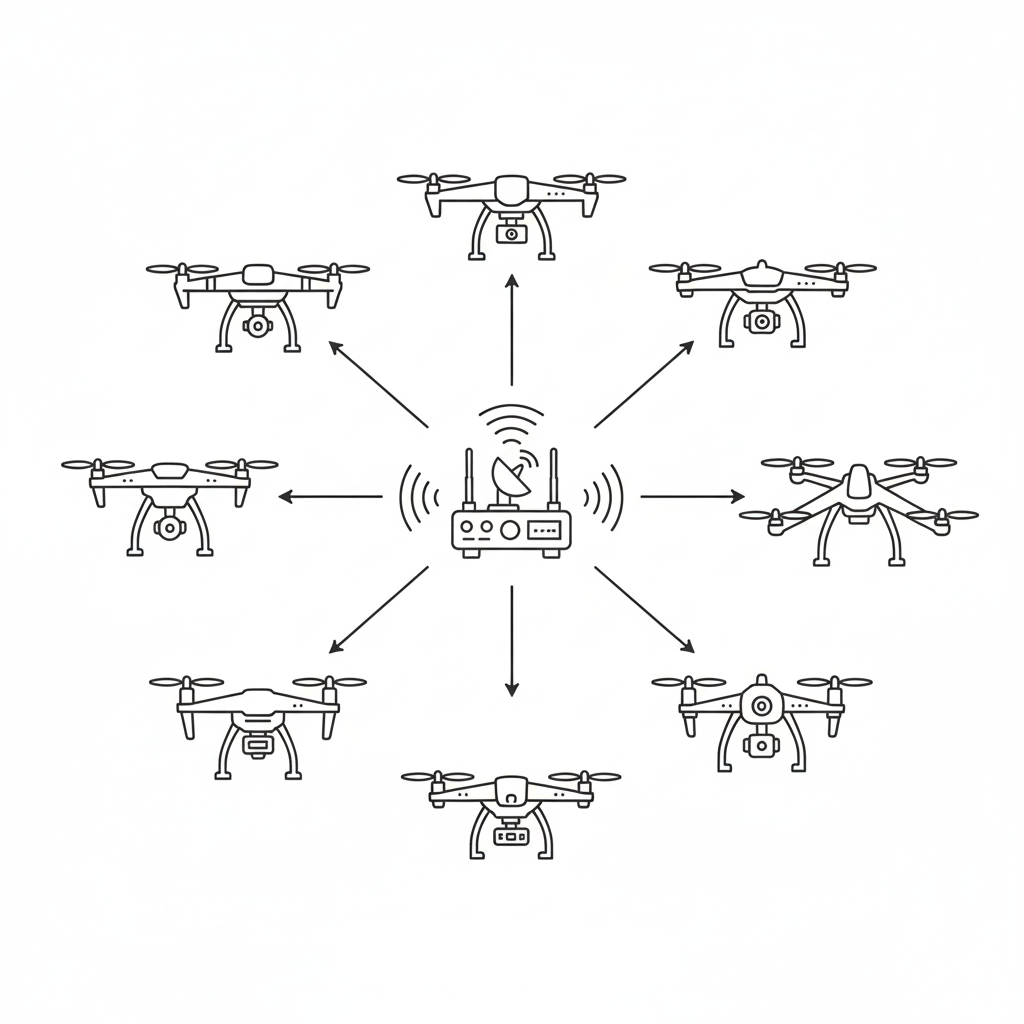
\includegraphics[width=1.0\linewidth]{images/controle centralizado.png}
    \caption{Representação do controle centralizado.}
    \label{fig:controle centralizado}
\end{figure}

\subsubsection{Controle Descentralizado e Distribuído}

No controle descentralizado, cada VANT toma decisões com base em informações locais, utilizando sensores embarcados ou comunicação com vizinhos próximos \citep{bu2024advancement}. Métodos como o \textit{Behavior-Based} e o \textit{Artificial Potential Field (APF)} são exemplos típicos dessa categoria.

Já no controle distribuído, embora não exista um centro de comando, há cooperação explícita entre os VANTs, que compartilham informações de estado para alcançar objetivos coletivos. Essa abordagem aumenta a robustez do sistema e melhora a escalabilidade, mas exige algoritmos mais complexos de consenso e sincronização \citep{bu2024advancement, ouyang2023formation}. Uma representação dessa arquitetura é mostrada na Figura~\ref{fig:controle distribuído}.

\begin{figure}[ht]
    \centering
    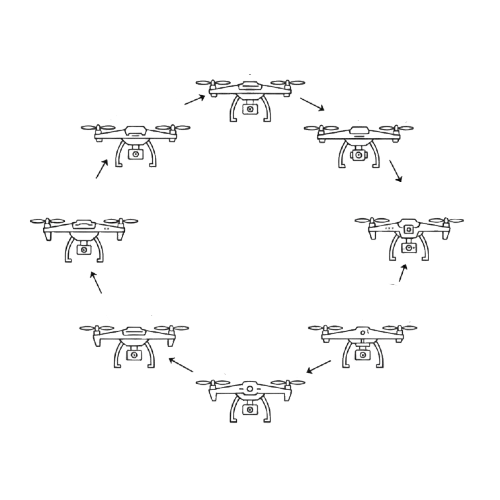
\includegraphics[width=1.0\linewidth]{images/controle distribuído rb1.png}
    \caption{Representação do controle distribuído.}
    \label{fig:controle distribuído}
\end{figure}

\subsubsection{Comparação entre Arquiteturas}

A Tabela~\ref{tab:arquiteturas-uavs} resume as principais características das arquiteturas de controle apresentadas anteriormente, destacando diferenças em robustez, escalabilidade e complexidade de implementação. Observa-se que a arquitetura centralizada apresenta baixa tolerância a falhas e escalabilidade limitada, porém sua implementação é conceitualmente mais simples. Por outro lado, arquiteturas descentralizadas ou distribuídas oferecem maior robustez e escalabilidade, mas exigem algoritmos de coordenação mais complexos, refletindo o trade-off clássico entre simplicidade de design e desempenho do sistema.


\begin{table*}[h!]
\centering
\caption{Comparação entre arquiteturas de controle em enxames de VANTs.}
\label{tab:arquiteturas-uavs}
\begin{tabular}{|p{3cm}|p{4cm}|p{3cm}|p{4cm}|}
\hline
\textbf{Estratégia} & \textbf{Robustez} & \textbf{Escalabilidade} & \textbf{Complexidade} \\ \hline
\textbf{Centralizada} & Baixa (alto risco de ponto único de falha) \citep{ouyang2023formation} & Limitada (sobrecarga computacional) \citep{bu2024advancement} & Simples (decisão unificada) \citep{bu2024advancement} \\ \hline
\textbf{Descentralizada e Distribuída} & Alta (forte tolerância a falhas) \citep{ouyang2023formation} & Alta (baseada em interações locais) \citep{bu2024advancement} & Elevada (coordenação e comunicação complexas) \citep{bu2024advancement} \\ \hline
\end{tabular}
\end{table*}


O controle distribuído tem se destacado como uma das tendências mais promissoras na pesquisa contemporânea, devido à sua robustez, flexibilidade e capacidade de escala \citep{ouyang2023formation}. Essa abordagem elimina a dependência de um ponto central e permite a coordenação emergente entre os veículos, sendo considerada a direção mais provável para o futuro das missões cooperativas com enxames de VANTs.

\subsection{Algoritmos de Formação de VANTs}

O controle de formação de VANTs consiste em coordenar o movimento de múltiplos veículos de modo que mantenham uma disposição espacial específica, geralmente representada por padrões geométricos como linha, V, triângulo ou diamante \citep{bu2024advancement}. Essa tarefa é central em aplicações cooperativas, como vigilância, mapeamento, busca e salvamento e monitoramento ambiental \citep{bu2024advancement, ouyang2023formation}.

Do ponto de vista matemático, a formação pode ser modelada considerando um conjunto de $N$ drones cuja posição linear é denotada por $p_i \in \mathbb{R}^n$. Aqui, $\mathbb{R}^n$ representa o espaço euclidiano de dimensão $n$, tipicamente $n = 2$ (espaço planar) ou $n = 3$ (espaço tridimensional).

As grandezas introduzidas nesta seção — $p_i$, $p_j$, $v_i$, $v_j$ — referem-se exclusivamente às componentes lineares da dinâmica dos VANTs. Variáveis angulares, tais como orientação e taxas de rotação, não são consideradas neste modelo específico, o qual foca apenas no comportamento translacional do sistema multiagente.

O objetivo do controle de formação é garantir que cada par de veículos $(i, j)$ mantenha sua separação e orientação relativa desejadas. Essa relação pode ser expressa pela seguinte condição de convergência:

\begin{equation}
\label{eq:formation_constraint}
\left\| (p_i - p_j) - d_{ij} \right\| \rightarrow 0, 
\qquad \forall \,(i,j) \in E,
\end{equation}

onde $p_{i}$ representa o vetor posição do drone $i$, $p_{j}$ representa o vetor posição do drone $j$, $d_{ij} \in \mathbb{R}^n$ é o vetor desejado de separação entre os drones $i$ e $j$, e $E$ representa o conjunto de arestas do grafo de vizinhanças que define quais veículos devem manter relações de formação entre si \citep{bu2024advancement, ouyang2023formation}.

Diversas abordagens de controle têm sido propostas para garantir a realização da formação, entre elas: \textit{Leader–Follower}, \textit{Virtual Structure}, \textit{Behavior-Based}, \textit{Consensus-Based} e \textit{Artificial Potential Fields}. Cada abordagem apresenta características próprias em relação à escalabilidade, robustez, dependência de comunicação e custo computacional \citep{bu2024advancement, ouyang2023formation}.


\subsubsection{Leader–Follower}

A abordagem \textit{Leader–Follower} baseia-se em uma estrutura hierárquica em que um ou mais VANTs atuam como líderes, definindo a trajetória global, enquanto os demais agentes (seguidores) mantêm posições relativas fixas em relação a eles \citep{liu2024leaderfollower}. Essa técnica é amplamente empregada por sua simplicidade e eficiência em pequenas formações \citep{bu2024advancement}.

Matematicamente, a posição desejada de um seguidor $i$ em relação a um líder $L$ pode ser descrita por

\begin{equation}
\label{eq:lf_desired_position}
p_i^{d}(t) = p_L(t) + R_L(t) \, d_i,
\end{equation}

onde $p_L(t)$ representa a posição linear do líder, e $R_L(t) \in SO(3)$ é a matriz de rotação associada à sua orientação. O conjunto $SO(3)$ denota o \textit{grupo especial ortogonal} de matrizes $3 \times 3$ que preservam normas e orientações, representando todas as possíveis rotações no espaço tridimensional. O vetor $d_i$ define a posição desejada do seguidor no referencial do líder, permanecendo fixo ao longo do tempo. A inclusão explícita de $R_L(t)$ garante que a formação mantenha sua geometria mesmo quando o líder altera sua orientação espacial.

O erro de formação é definido como

\begin{equation}
\label{eq:lf_error}
e_i(t) = p_i^{d}(t) - p_i(t) = p_L(t) + R_L(t)d_i - p_i(t),
\end{equation}

e a lei de controle de velocidade, considerando um esquema proporcional-derivativo (PD) com \textit{feed-forward} da velocidade do líder, é dada por

\begin{equation}
\label{eq:lf_control_law}
u_i(t) = v_L(t) + K_p e_i(t) + K_d \big(v_L(t) - v_i(t)\big),
\end{equation}

em que $u_i(t)$ é o comando de velocidade do seguidor, $v_L(t) = \dot{p}_L(t)$ é a velocidade linear do líder, e $K_p, K_d > 0$ são ganhos de controle responsáveis pela dinâmica da resposta de formação. Essa formulação assegura que os seguidores mantenham a separação e orientação desejadas em relação ao líder, acompanhando suavemente mudanças na trajetória global.

Uma representação esquemática da abordagem Leader–Follower é apresentada na Figura~\ref{fig:leader-follower}.

\begin{figure}[ht]
    \centering
    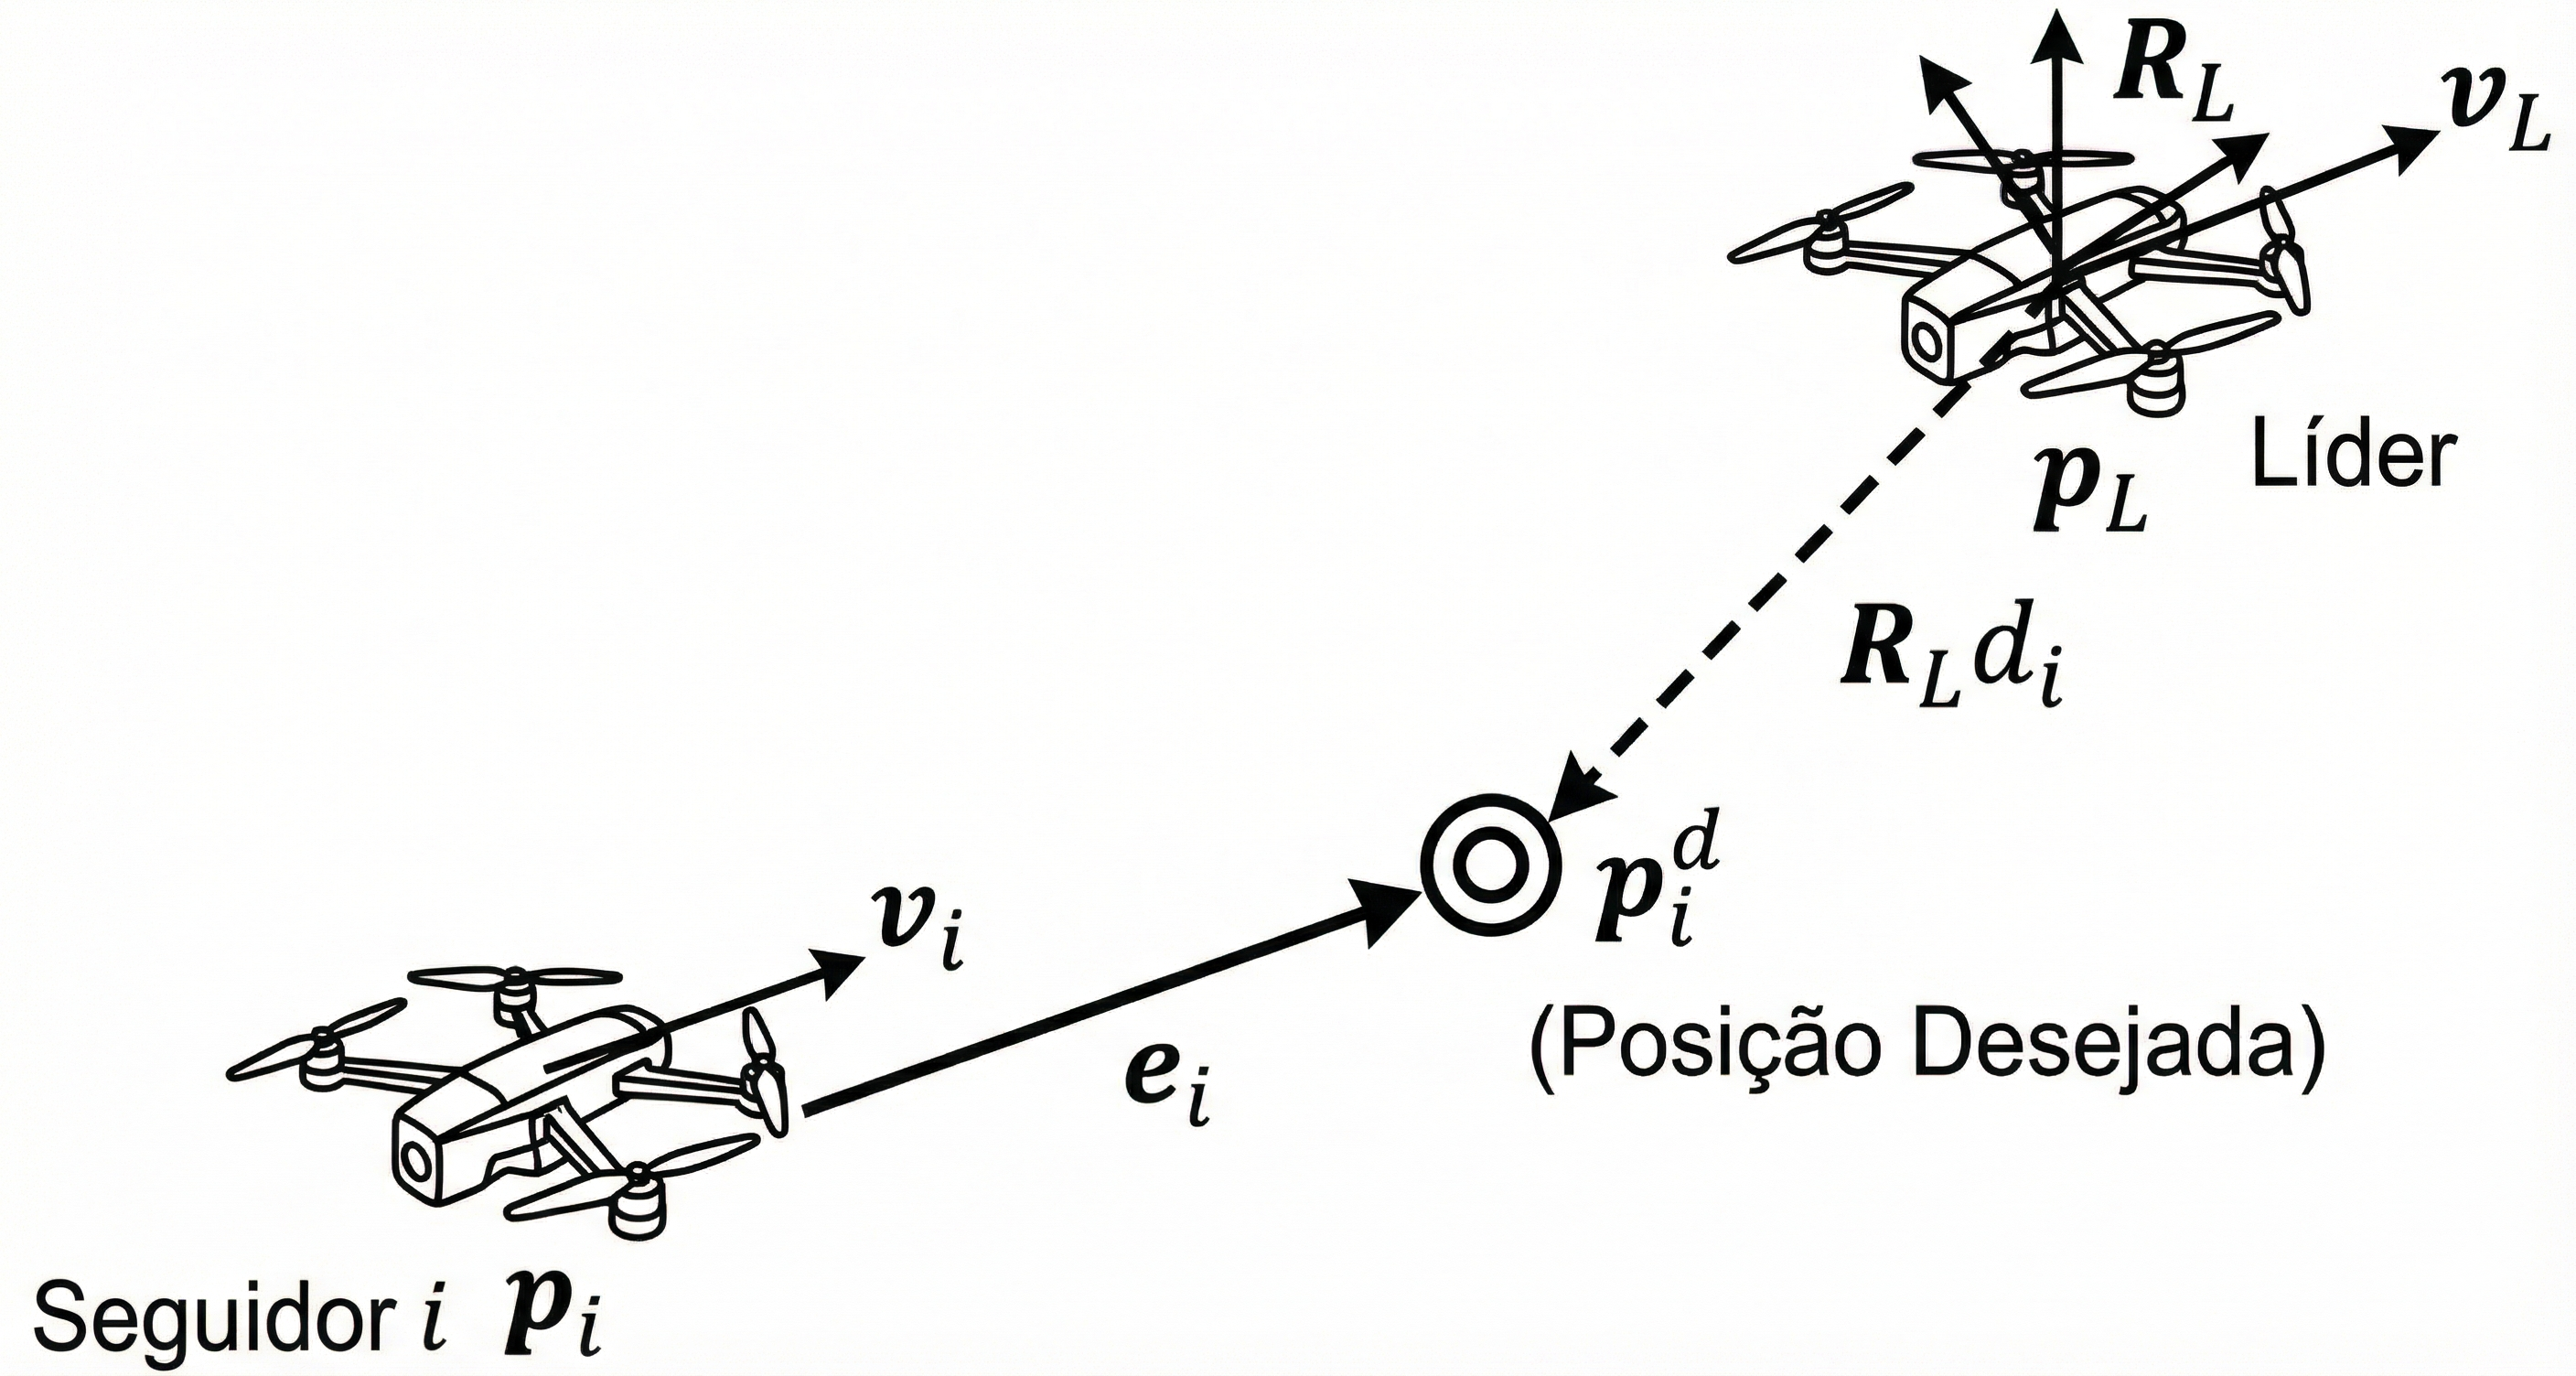
\includegraphics[width=0.7\linewidth]{images/Leader-Follower_pt.png}
    \caption{Representação do algoritmo Leader--Follower.}
    \label{fig:leader-follower}
\end{figure}

Apesar de sua simplicidade, o método é sensível à perda de comunicação ou falha do líder, o que pode comprometer a coesão do grupo. Abordagens mais recentes buscam mitigar essas limitações por meio de múltiplos líderes ou estratégias distribuídas de controle cooperativo.


\subsubsection{Virtual Structure}

Na estratégia \textit{Virtual Structure}, o grupo de VANTs é tratado como uma única estrutura rígida virtual, em que cada veículo ocupa uma posição fixa pré-definida dentro dessa estrutura \citep{bu2024advancement, askari2015virtualstructure}. O enxame, então, desloca-se como uma entidade unificada, preservando forma e orientação com elevada precisão.

Seja $p_v(t) \in \mathbb{R}^3$ a posição do centro da estrutura virtual e $R_v(t) \in SO(3)$ sua matriz de rotação, que define a orientação global da formação. Cada VANT $i$ possui um vetor $r_i^{VS}$ que especifica sua posição relativa fixa dentro da estrutura. Assim, a posição desejada do VANT $i$ é:

\begin{equation}
p_i^{d}(t) = p_v(t) + R_v(t)\, r_i^{VS}
\end{equation}

A velocidade desejada segue da cinemática de corpo rígido:

\begin{equation}
v_i^{d}(t) = v_v(t) + \omega_v(t) \times \big( R_v(t)\, r_i^{VS} \big)
\end{equation}



onde $v_v(t)$ é a velocidade linear da estrutura virtual. O termo $\times$ denota explicitamente o produto vetorial entre a velocidade angular da estrutura virtual e a posição relativa do VANT expressa no referencial global.

O controle de posição e velocidade de cada VANT é definido por uma lei de controle proporcional-derivativa (PD), dada por:

\begin{equation}
u_i = K_p (p_i^{d} - p_i) + K_d (v_i^{d} - v_i)
\end{equation}

onde $u_i$ representa o vetor de aceleração de controle do VANT $i$, e $K_p$, $K_d$ são matrizes de ganhos proporcionais e derivativos, respectivamente. Substituindo $v_i^{d}(t)$, tem-se explicitamente:

\begin{equation}
u_i = K_p (p_v + R_v r_i^{VS} - p_i) + K_d (v_v + \omega_v \times R_v r_i^{VS} - v_i)
\end{equation}

Essa lei de controle assegura que cada VANT siga rigidamente o movimento da estrutura virtual, compensando desvios de posição e velocidade em relação à sua referência local dentro do corpo virtual.

Assumindo uma dinâmica de segunda ordem $\ddot{p}_i = u_i$, o erro de posição $e_i = p_i^{d} - p_i$ evolui segundo:

\begin{equation}
\ddot{e}_i + K_d \dot{e}_i + K_p e_i = 0
\end{equation}

o que caracteriza um sistema linear de segunda ordem estável se $K_p > 0$ e $K_d > 0$, garantindo convergência exponencial do erro para zero.

A principal vantagem dessa abordagem é a manutenção precisa da geometria da formação, mesmo em manobras complexas. Entretanto, ela requer sincronização e comunicação global entre os VANTs para garantir consistência no estado da estrutura virtual, o que pode limitar sua aplicação em cenários com comunicação intermitente ou ambientes altamente dinâmicos \citep{bu2024advancement, ouyang2023formation}.




\subsubsection{Behavior-Based}

A abordagem \textit{Behavior-Based} fundamenta-se em regras locais simples, inspiradas em sistemas biológicos como bandos de aves e cardumes de peixes \citep{balch2002behaviorbased}. Cada VANT ajusta seu movimento de forma autônoma com base em informações provenientes apenas de seus vizinhos mais próximos, seguindo comportamentos fundamentais de \textit{separação}, \textit{coesão}, \textit{alinhamento} e, em algumas aplicações, \textit{busca por objetivo} (\textit{goal seeking}) \citep{ouyang2023formation, reynolds1987flocks}.

A força de controle total aplicada ao agente $i$ é obtida pela soma ponderada dos vetores de cada comportamento:

\begin{equation}
u_i = w_s f_{sep,i} + w_c f_{coh,i} + w_a f_{ali,i} + w_g f_{goal,i}
\end{equation}

onde $w_s$, $w_c$, $w_a$ e $w_g$ são os pesos que determinam a influência relativa do comportamento de Separação, Coesão, Alinhamento e Busca por objetivo, respectivamente. Os vetores de controle são definidos como:

\begin{equation}
\begin{aligned}
f_{sep,i} &= \sum_{j \in N_i} \frac{p_i - p_j}{\|p_i - p_j\|^2} && \text{(Separação)} \\[6pt]
f_{coh,i} &= \frac{1}{|N_i|}\sum_{j \in N_i}(p_j - p_i) && \text{(Coesão)} \\[6pt]
f_{ali,i} &= \frac{1}{|N_i|}\sum_{j \in N_i}(v_j - v_i) && \text{(Alinhamento)} \\[6pt]
f_{goal,i} &= p_{goal} - p_i && \text{(Busca por objetivo)}
\end{aligned}
\end{equation}

O comportamento de \textit{separação} evita colisões e mantém espaçamento mínimo seguro entre os VANTs; o de \textit{coesão} busca preservar a unidade do grupo; o de \textit{alinhamento} sincroniza a direção de voo com a média dos vizinhos; e o de \textit{busca por objetivo} conduz o enxame a um alvo ou trajetória desejada.

A dinâmica de cada agente é descrita por:

\begin{equation}
\dot{p}_i = v_i, \quad \dot{v}_i = u_i
\end{equation}

onde $p_i$ e $v_i$ são, respectivamente, a posição linear e a velocidade linear do VANT $i$. Assim, o vetor $u_i$ representa a aceleração desejada calculada a partir da combinação dos comportamentos locais.

Essa formulação resulta em um sistema de controle totalmente distribuído, no qual o comportamento coletivo emerge das interações locais entre agentes. Tal característica garante escalabilidade e robustez a falhas de comunicação, mas dificulta a manutenção de formações geométricas rígidas e a obtenção de estabilidade formal em cenários complexos \citep{bu2024advancement, ouyang2023formation}.

\subsubsection{Consensus-Based}

Os métodos \textit{Consensus-Based} têm como objetivo permitir que todos os VANTs atinjam um acordo (\textit{consenso}) sobre variáveis de estado, como posição, velocidade ou orientação, utilizando apenas informações locais de vizinhança \citep{bu2024advancement, ouyang2023formation, olfati2007consensus, ren2008distributed}. 

A topologia de comunicação entre os VANTs é representada por um grafo direcionado \(\mathcal{G} = (\mathcal{V}, \mathcal{E})\), onde \(\mathcal{V} = \{1, 2, \dots, N\}\) é o conjunto de agentes e \(\mathcal{E} \subseteq \mathcal{V} \times \mathcal{V}\) define as conexões entre eles.  
A matriz de adjacência \(A = [a_{ij}]\in\mathbb{R}^{N\times N}\) é definida por

\begin{equation}
a_{ij} =
\begin{cases}
>0, & \text{se existe aresta }(j,i)\in\mathcal{E},\\[4pt]
0,  & \text{caso contrário.}
\end{cases}
\end{equation}


Ou seja, a entrada \(a_{ij}\) representa o peso com que a informação do agente \(j\) é considerada pelo agente \(i\). Para cada agente \(i\) definimos o grau (in-degree) como

\begin{equation}
d_i = \sum_{j=1}^{N} a_{ij},
\end{equation}

e a matriz diagonal dos graus \(D=\mathrm{diag}(d_1,\dots,d_N)\). A matriz Laplaciana é então definida por \(L = D - A\).

Além disso, denotamos por \(\mathcal{N}_i\) o conjunto de vizinhos que enviam informação ao agente \(i\), isto é

\begin{equation}
\mathcal{N}_i = \{\, j \in \mathcal{V} \mid a_{ij} > 0 \,\},
\end{equation}

(às vezes chamado de \emph{in-neighborhood} de \(i\)). A notação \(\sum_{j\in\mathcal{N}_i}\) indica somas apenas sobre esses vizinhos.

\paragraph{Modelagem para agentes de primeira ordem.}
Considerando que cada agente \(i\) possui um estado \(x_i(t)\) e que sua dinâmica é dada por \(\dot{x}_i = u_i\), o controle de consenso é expresso por:

\begin{equation}
u_i = -\sum_{j \in \mathcal{N}_i} a_{ij} (x_i - x_j).
\end{equation}

Substituindo em \(\dot{x}_i = u_i\), tem-se a forma dinâmica contínua:

\begin{equation}
\dot{x}_i = -\sum_{j \in \mathcal{N}_i} a_{ij} (x_i - x_j),
\end{equation}

ou, de forma vetorial compacta:

\begin{equation}
\dot{x} = -Lx,
\end{equation}

onde \(x = [x_1, x_2, \dots, x_N]^T\). Quando o grafo é fortemente conexo, o sistema garante a convergência para o consenso global:

\begin{equation}
\lim_{t \to \infty} (x_i(t) - x_j(t)) = 0, \quad \forall i,j.
\end{equation}

\paragraph{Modelagem para agentes de segunda ordem.}
Em sistemas mais realistas, como enxames de VANTs, é necessário considerar tanto a posição \(p_i\) quanto a velocidade \(v_i\) de cada agente. Assim, a dinâmica de segunda ordem é dada por:

\begin{equation}
\begin{cases}
\dot{p}_i = v_i,\\[4pt]
\dot{v}_i = u_i.
\end{cases}
\end{equation}

O controle de consenso estendido para esse caso pode ser expresso como:

\begin{equation}
u_i = -k_p \sum_{j \in \mathcal{N}_i} a_{ij}(p_i - p_j) - k_v \sum_{j \in \mathcal{N}_i} a_{ij}(v_i - v_j),
\end{equation}

em que \(k_p\) e \(k_v\) são ganhos de acoplamento que determinam a velocidade de convergência da formação. Sob condições de conectividade adequadas do grafo, o sistema tende a garantir:

\begin{equation}
\lim_{t \to \infty} (p_i(t) - p_j(t)) = 0, \quad \lim_{t \to \infty} (v_i(t) - v_j(t)) = 0, \quad \forall i,j,
\end{equation}

ou seja, todos os VANTs convergem para a mesma trajetória e velocidade, atingindo consenso tanto em posição quanto em movimento.

Essa abordagem apresenta uma base teórica sólida e comprovada estabilidade quando o grafo de comunicação é conexo. Sua simplicidade, robustez e escalabilidade tornam o método \textit{Consensus-Based} amplamente utilizado em aplicações de coordenação distribuída, controle de formação e sincronização em redes multiagente \citep{olfati2007consensus, ren2008distributed}.


\subsubsection{Artificial Potential Fields}

O método dos \textit{Artificial Potential Fields} (APF) propõe o uso de campos de potencial artificiais para gerar forças virtuais de atração e repulsão que guiam o movimento dos agentes de forma contínua e descentralizada \citep{khatib1986real, bu2024advancement, ouyang2023formation}. Nesse contexto, o ambiente é modelado como um campo energético, em que o objetivo atua como uma fonte atrativa e os obstáculos ou demais VANTs funcionam como fontes repulsivas.

O potencial total associado ao agente $i$ é definido por:

\begin{equation}
U_i(p_i) = U_{att}(p_i) + U_{rep}(p_i)
\end{equation}

em que o termo atrativo $U_{att}(p_i)$ direciona o VANT para o alvo e o termo repulsivo $U_{rep}(p_i)$ evita colisões com obstáculos e vizinhos próximos. O potencial atrativo é geralmente modelado de forma quadrática:

\begin{equation}
U_{att}(p_i) = \frac{1}{2} k_{att} \|p_i - p_{goal}\|^2
\end{equation}

onde $k_{att} > 0$ representa o ganho de atração e $p_{goal}$ a posição desejada. Já o potencial repulsivo atua apenas dentro de uma distância de influência $d_0$, sendo dado por:

\begin{equation}
U_{rep}(p_i) =
\frac{1}{2} k_{rep} 
\sum_{j \in N_i}
\left(
\frac{1}{\|p_i - p_j\|} - \frac{1}{d_0}
\right)^2
\mathbb{I}_{\|p_i - p_j\| < d_0}
\end{equation}

onde $k_{rep} > 0$ é o ganho de repulsão, $N_i$ representa o conjunto de vizinhos do agente $i$, e $\mathbb{I}$ é a função indicadora, que vale 1 quando a condição é verdadeira e 0 caso contrário.

A força resultante que governa o movimento do agente é obtida pelo gradiente negativo do potencial total:

\begin{equation}
f_i = -\nabla U_i = f_{att,i} + f_{rep,i}
\end{equation}

com:

\begin{equation}
\begin{split}
f_{att,i} &= -k_{att}(p_i - p_{goal}), \\
f_{rep,i} &= 
\sum_{j \in N_i} k_{rep}
\left(\frac{1}{\|p_i - p_j\|} - \frac{1}{d_0}\right)
\\
&\quad\times
\frac{1}{\|p_i - p_j\|^3}(p_i - p_j)
\mathbb{I}_{\|p_i - p_j\| < d_0}
\end{split}
\end{equation}

A dinâmica de movimento pode ser modelada por:

\begin{equation}
\dot{p}_i = v_i, \quad
\dot{v}_i = f_i
\end{equation}

de modo que cada VANT ajusta sua aceleração de acordo com o gradiente do campo de potencial. Essa formulação permite que as formações se reorganizem em tempo real e evitem colisões, mesmo em ambientes dinâmicos. No entanto, o método pode apresentar limitações devido à presença de mínimos locais — situações em que o potencial total apresenta pontos de equilíbrio indesejados que impedem a convergência ao objetivo \citep{khatib1986real, bu2024advancement, ouyang2023formation}. Uma representação da abordagem APF é mostrada na Figura~\ref{fig:APF}.

\begin{figure}[ht]
    \centering
    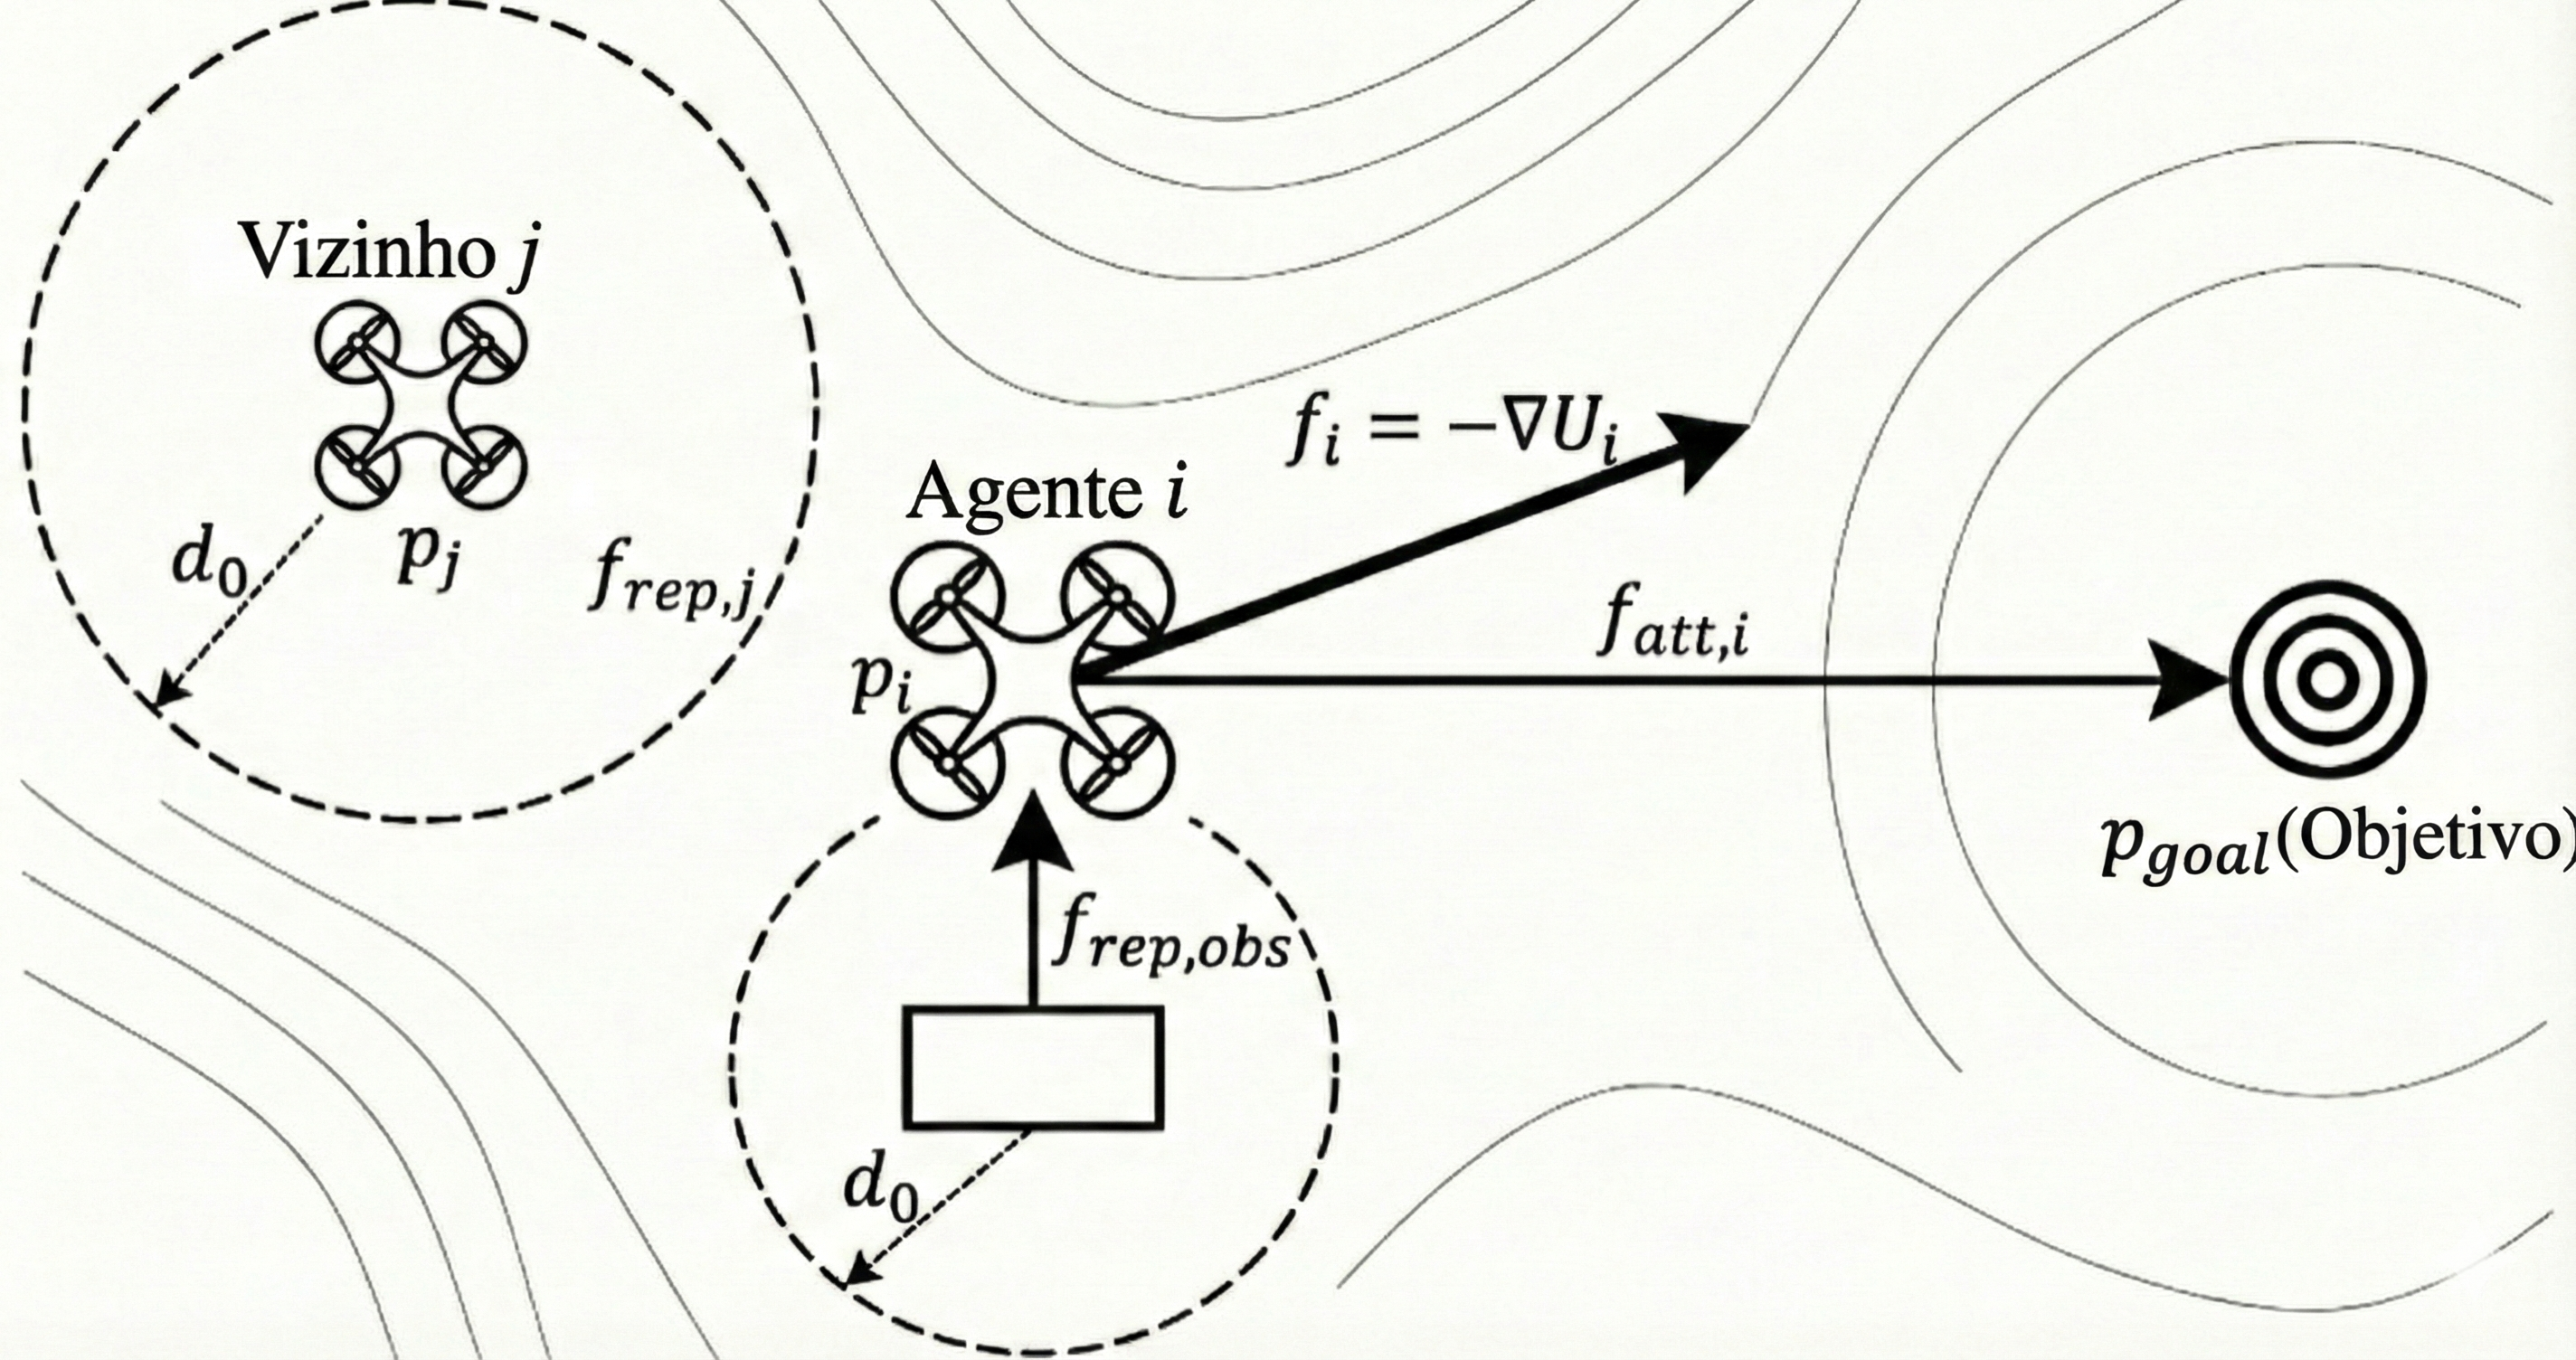
\includegraphics[width=1.0\linewidth]{images/APF_pt.png}
    \caption{Representação do algoritmo APF.}
    \label{fig:APF}
\end{figure}

\subsubsection*{Comparação Geral}

Cada uma dessas abordagens apresenta vantagens específicas. Os métodos \textit{Leader–Follower} e \textit{Virtual Structure} são indicados para formações bem definidas e controladas centralmente, enquanto as estratégias \textit{Behavior-Based}, \textit{Consensus-Based} e \textit{Artificial Potential Fields} são mais adequadas para ambientes dinâmicos e distribuídos. Em sistemas reais, é comum a combinação híbrida entre métodos, buscando equilibrar estabilidade, escalabilidade e adaptabilidade \citep{bu2024advancement, ouyang2023formation}.

\subsection{Comunicação e Coordenação em Enxames de VANTs}

A comunicação é um elemento essencial para a coordenação eficiente de enxames de VANTs. Para permitir a troca contínua de informações de estado, sensores e planos de voo, os VANTs frequentemente operam em redes ad hoc, conhecidas como FANETs (Flying Ad Hoc Networks) \citep{khan2017fanet, hong2020swarm}.

As FANETs diferenciam-se de redes terrestres tradicionais por características como alta mobilidade, auto-organização e ausência de controle centralizado. A dinâmica tridimensional dos VANTs, associada à sua velocidade de deslocamento (30 a 460 km/h), resulta em rápidas variações na topologia da rede, o que impõe desafios de conectividade e exige protocolos de comunicação resilientes \citep{khan2017fanet}.

Protocolos de comunicação comuns incluem Wi-Fi, UWB (Ultra-Wideband) e Bluetooth, selecionados conforme o alcance, largura de banda e consumo de energia requeridos \citep{chung2018survey}. A comunicação entre VANTs pode ser representada por meio de grafos direcionados ou não direcionados, em que cada nó representa um veículo e cada aresta representa um canal de comunicação ativo \citep{ren2007consensus}. Essa modelagem é particularmente útil para o desenvolvimento de algoritmos de consenso e controle distribuído.

A comunicação e a coordenação são pilares fundamentais para o funcionamento de sistemas cooperativos de VANTs (Veículos Aéreos Não Tripulados). Esses elementos determinam não apenas a eficiência das formações, mas também a robustez e escalabilidade das missões em ambientes dinâmicos e distribuídos \citep{ren2007consensus, Young-Min2018, khaliq2021}.

Através de protocolos de comunicação específicos, como o \textit{MAVLink}, e estruturas de software distribuídas, como o \textit{ROS} (Robot Operating System) e o \textit{ROS2} (segunda geração do Robot Operating System, baseada em DDS e arquitetura totalmente distribuída), é possível garantir a troca contínua de dados entre os veículos e entre estes e a estação de controle \citep{ziming2023}. No entanto, para que a cooperação ocorra de maneira eficiente, é essencial que a rede de comunicação suporte o compartilhamento rápido e confiável de informações — algo desafiador em redes altamente dinâmicas, como as \textit{FANETs} (Flying Ad hoc Networks), sujeitas à latência, perdas de pacotes e instabilidade topológica \citep{inam2017, hong2020swarm, ouyang2023formation}.

\subsubsection{Protocolos de VANTs e Arquiteturas de Comunicação}

O protocolo \textit{MAVLink}, amplamente utilizado em sistemas \textit{open-source} como PX4 e ArduPilot, provê uma camada leve de comunicação baseada em mensagens que permite a troca de dados entre o sistema de controle de voo e a estação terrestre \citep{Young-Min2018}. Em conjunto, o \textit{ROS} e o \textit{ROS2} fornecem uma infraestrutura modular e distribuída que viabiliza a integração de múltiplos agentes, sensores e atuadores, promovendo interoperabilidade entre diferentes sistemas e linguagens \citep{khaliq2021, ziming2023}.

Essas tecnologias permitem o desenvolvimento de arquiteturas descentralizadas, nas quais cada VANT pode atuar como um nó inteligente em uma rede distribuída, trocando informações localmente com seus vizinhos e ajustando seu comportamento coletivo com base em protocolos de consenso \citep{ren2007consensus, bu2024advancement}. O uso do \textit{DDS} (Data Distribution Service) em \textit{ROS2} melhora a escalabilidade e a confiabilidade dessas trocas, tornando o sistema mais tolerante a falhas de comunicação.

\subsubsection{Limitações e Desafios de Comunicação}

Apesar do avanço nos protocolos e arquiteturas, a comunicação entre VANTs permanece sujeita a limitações significativas. A natureza tridimensional e dinâmica das \textit{FANETs} impõe desafios quanto à latência, perda de pacotes e vulnerabilidade a ataques de rede, como \textit{ICMP flooding} e negação de serviço (DoS) \citep{Young-Min2018}. Esses fatores podem comprometer a estabilidade de formações e causar falhas críticas em missões coordenadas.

Estudos experimentais mostraram que ataques de saturação podem aumentar a variância do tempo de recepção de dados em mais de 30 vezes, afetando diretamente o desempenho dos controladores de formação \citep{Young-Min2018}. Além disso, a degradação do sinal (RSSI) e a quebra de links em redes \textit{mesh} reduzem a capacidade de sincronização entre os drones, exigindo estratégias adaptativas de roteamento e controle \citep{hong2020swarm, khaliq2021}.

\subsection{Simulação de Enxames de VANTs}

As plataformas de simulação são ferramentas essenciais no desenvolvimento e validação de estratégias de controle cooperativo e comunicação entre VANTs \citep{khaliq2021, ziming2023}. Elas permitem testar algoritmos de formação, sincronização e evasão de obstáculos em ambientes virtuais, reduzindo custos e riscos associados a testes reais.

\subsubsection{Plataformas e Motores de Simulação}

Simuladores como \textit{Gazebo}, \textit{Webots}, \textit{CoppeliaSim} e o \textit{SITL PX4} fornecem ambientes tridimensionais realistas para a modelagem de cenários de voo e formação \citep{ziming2023}. O \textit{Gazebo}, por exemplo, integra-se ao \textit{ROS}/ROS~2 para simulações \textit{Software-In-The-Loop} (SIL) e \textit{Hardware-In-The-Loop} (HIL), utilizando motores de física como ODE, Bullet e DART \citep{khaliq2021, GazeboClassic2024, GazeboPhysicsEngines2024}. Estudos comparativos indicam que o \textit{Gazebo} se destaca entre os simuladores 3D integrados ao ROS em cenários multi-robô, mantendo fatores de tempo-real adequados mesmo com múltiplos agentes \citep{Noori2017}.

Já o \textit{Webots} destaca-se pela flexibilidade e suporte a sensores complexos, sendo amplamente utilizado em experimentos de enxames e controle distribuído \citep{ziming2023}. Tais simuladores não apenas reproduzem o comportamento físico dos VANTs, mas também emulam suas redes de comunicação via MAVLink e ROS, permitindo testes completos de sistemas multiagentes \citep{Ponniah2019, Meighan2025}.

\subsubsection{Comunicação e Modelagem em Simulação}

Durante simulações cooperativas, o MAVLink atua como o protocolo de mensageria entre os nós simulados, e o MAVROS realiza a interface entre o sistema de controle e os tópicos ROS \citep{khaliq2021, Koubaa2019, MAVROS2024}. Essa configuração possibilita a criação de redes \textit{mesh} distribuídas, nas quais cada VANT emulado executa seu próprio nó ROS/ROS~2 e interage com os demais por meio de mensagens trocadas em tempo real \citep{ROS2Design2022, ROS2QoS2024}.

Além disso, a modelagem de sensores e ambientes permite testar a robustez dos algoritmos em condições realistas, incluindo ruído, atraso de comunicação e falhas de hardware simuladas \citep{ziming2023, PX4SITL2024}. Essa integração entre simulação física, autopiloto em modo SITL e rede distribuída fornece uma base sólida para o desenvolvimento de estratégias de coordenação robustas \citep{Ponniah2019, Noori2017}.



\subsection{Síntese e Direcionamento do Trabalho}

A fundamentação teórica apresentada integrou os principais conceitos relacionados à comunicação, coordenação, simulação e controle de formação em enxames de VANTs, delineando o panorama atual das tecnologias e desafios envolvidos no desenvolvimento de sistemas cooperativos autônomos.

Os protocolos de comunicação, como o \textit{MAVLink} e o \textit{ROS/ROS2}, fornecem a base para a interoperabilidade e sincronização entre múltiplos agentes, permitindo a troca de informações de estado e o controle distribuído. Sobre essa infraestrutura, os algoritmos de formação — como os baseados em consenso, comportamento e estruturas virtuais — determinam a dinâmica coletiva dos VANTs, regulando como o grupo se organiza, mantém coesão e responde a perturbações externas. Já as plataformas de simulação, como o \textit{Gazebo} e o \textit{SITL PX4}, tornam possível testar e validar essas estratégias em cenários controlados, antes de sua aplicação em experimentos reais \citep{ouyang2023formation, bu2024advancement, khaliq2021}.

Com base nessa revisão, este trabalho propõe investigar de forma comparativa o desempenho de diferentes algoritmos e arquiteturas de controle de formação em diferentes cenários. O foco não se limita à reprodução de resultados consolidados, mas à análise crítica da aplicabilidade de cada método sob condições diversas — como a presença de obstáculos, variações de topologia de comunicação e ajustes de parâmetros dinâmicos.

Além disso, será explorada a hibridização de algoritmos, combinando propriedades de estratégias como \textit{Leader–Follower}, \textit{Consensus-Based} e \textit{Artificial Potential Fields (APF)}. Essa abordagem busca identificar configurações que maximizem a estabilidade da formação e a eficiência da comunicação, sem comprometer a adaptabilidade e a robustez do enxame. O objetivo final é definir uma arquitetura de sistema que permita a coordenação autônoma, eficiente e adaptável de múltiplos drones em diferentes cenários.




\section{Metodologia}

A metodologia adotada neste trabalho foi estruturada para permitir uma análise comparativa rigorosa entre diferentes algoritmos de controle cooperativo de formação de VANTs (Veículos Aéreos Não Tripulados). A abordagem é experimental, quantitativa e fundamentada em simulações computacionais, de modo a garantir reprodutibilidade, isolamento de variáveis e segurança no estudo de comportamento coletivo. O processo foi dividido em quatro etapas principais: (i) definição dos algoritmos e cenários; (ii) implementação dos modelos de controle; (iii) execução das simulações; e (iv) análise dos resultados.

Inicialmente, serão selecionados os algoritmos amplamente utilizados em controle cooperativo de formação. Entre eles, temos:

\begin{itemize}
    \item \textbf{Leader–Follower}: estrutura hierárquica em que um agente líder define a trajetória e os seguidores ajustam suas posições relativas;
    \item \textbf{Consensus-Based}: cada agente atualiza seu estado com base nos vizinhos, buscando convergência coletiva;
    \item \textbf{Behavior-Based}: comportamentos individuais (coesão, separação, alinhamento) geram padrões emergentes;
    \item \textbf{Virtual Structure}: a formação é tratada como uma estrutura rígida virtual, com posições relativas predefinidas;
    \item \textbf{Artificial Potential Fields (APF)}: o movimento decorre de forças atrativas e repulsivas que moldam o posicionamento desejado.
\end{itemize}

Com o objetivo de investigar potenciais melhorias no desempenho, também serão consideradas combinações híbridas de algoritmos, explorando complementaridades entre abordagens — por exemplo, a combinação entre \textit{Consensus-Based} e \textit{APF} para simultaneamente manter coesão e evitar colisões.

As simulações serão realizadas utilizando o simulador \textit{Gazebo}, integrado ao middleware \textit{ROS2} e ao firmware PX4 Autopilot em modo SITL (\textit{Software-In-The-Loop}), conforme ilustrado na Figura~\ref{fig:Arquitetura de simulação}. Essa escolha se justifica por três razões principais: (i) o \textit{Gazebo} fornece um ambiente tridimensional realista com motores de física robustos, permitindo simulação de dinâmicas e colisões com alta fidelidade; (ii) o \textit{ROS2} possibilita arquitetura modular, comunicação determinística e suporte nativo a sistemas distribuídos, características essenciais para experimentos com múltiplos agentes; e (iii) o PX4 SITL permite emular o comportamento do autopiloto real, utilizando o protocolo MAVLink para comandar cada VANT, o que preserva a compatibilidade com sistemas embarcados reais e facilita a futura transição para testes em campo. As implementações dos controladores serão desenvolvidas em \textit{Python}, com o uso de \textit{NumPy} para cálculos numéricos e \textit{Matplotlib} para análise gráfica.

\begin{figure*}[ht]
    \centering
    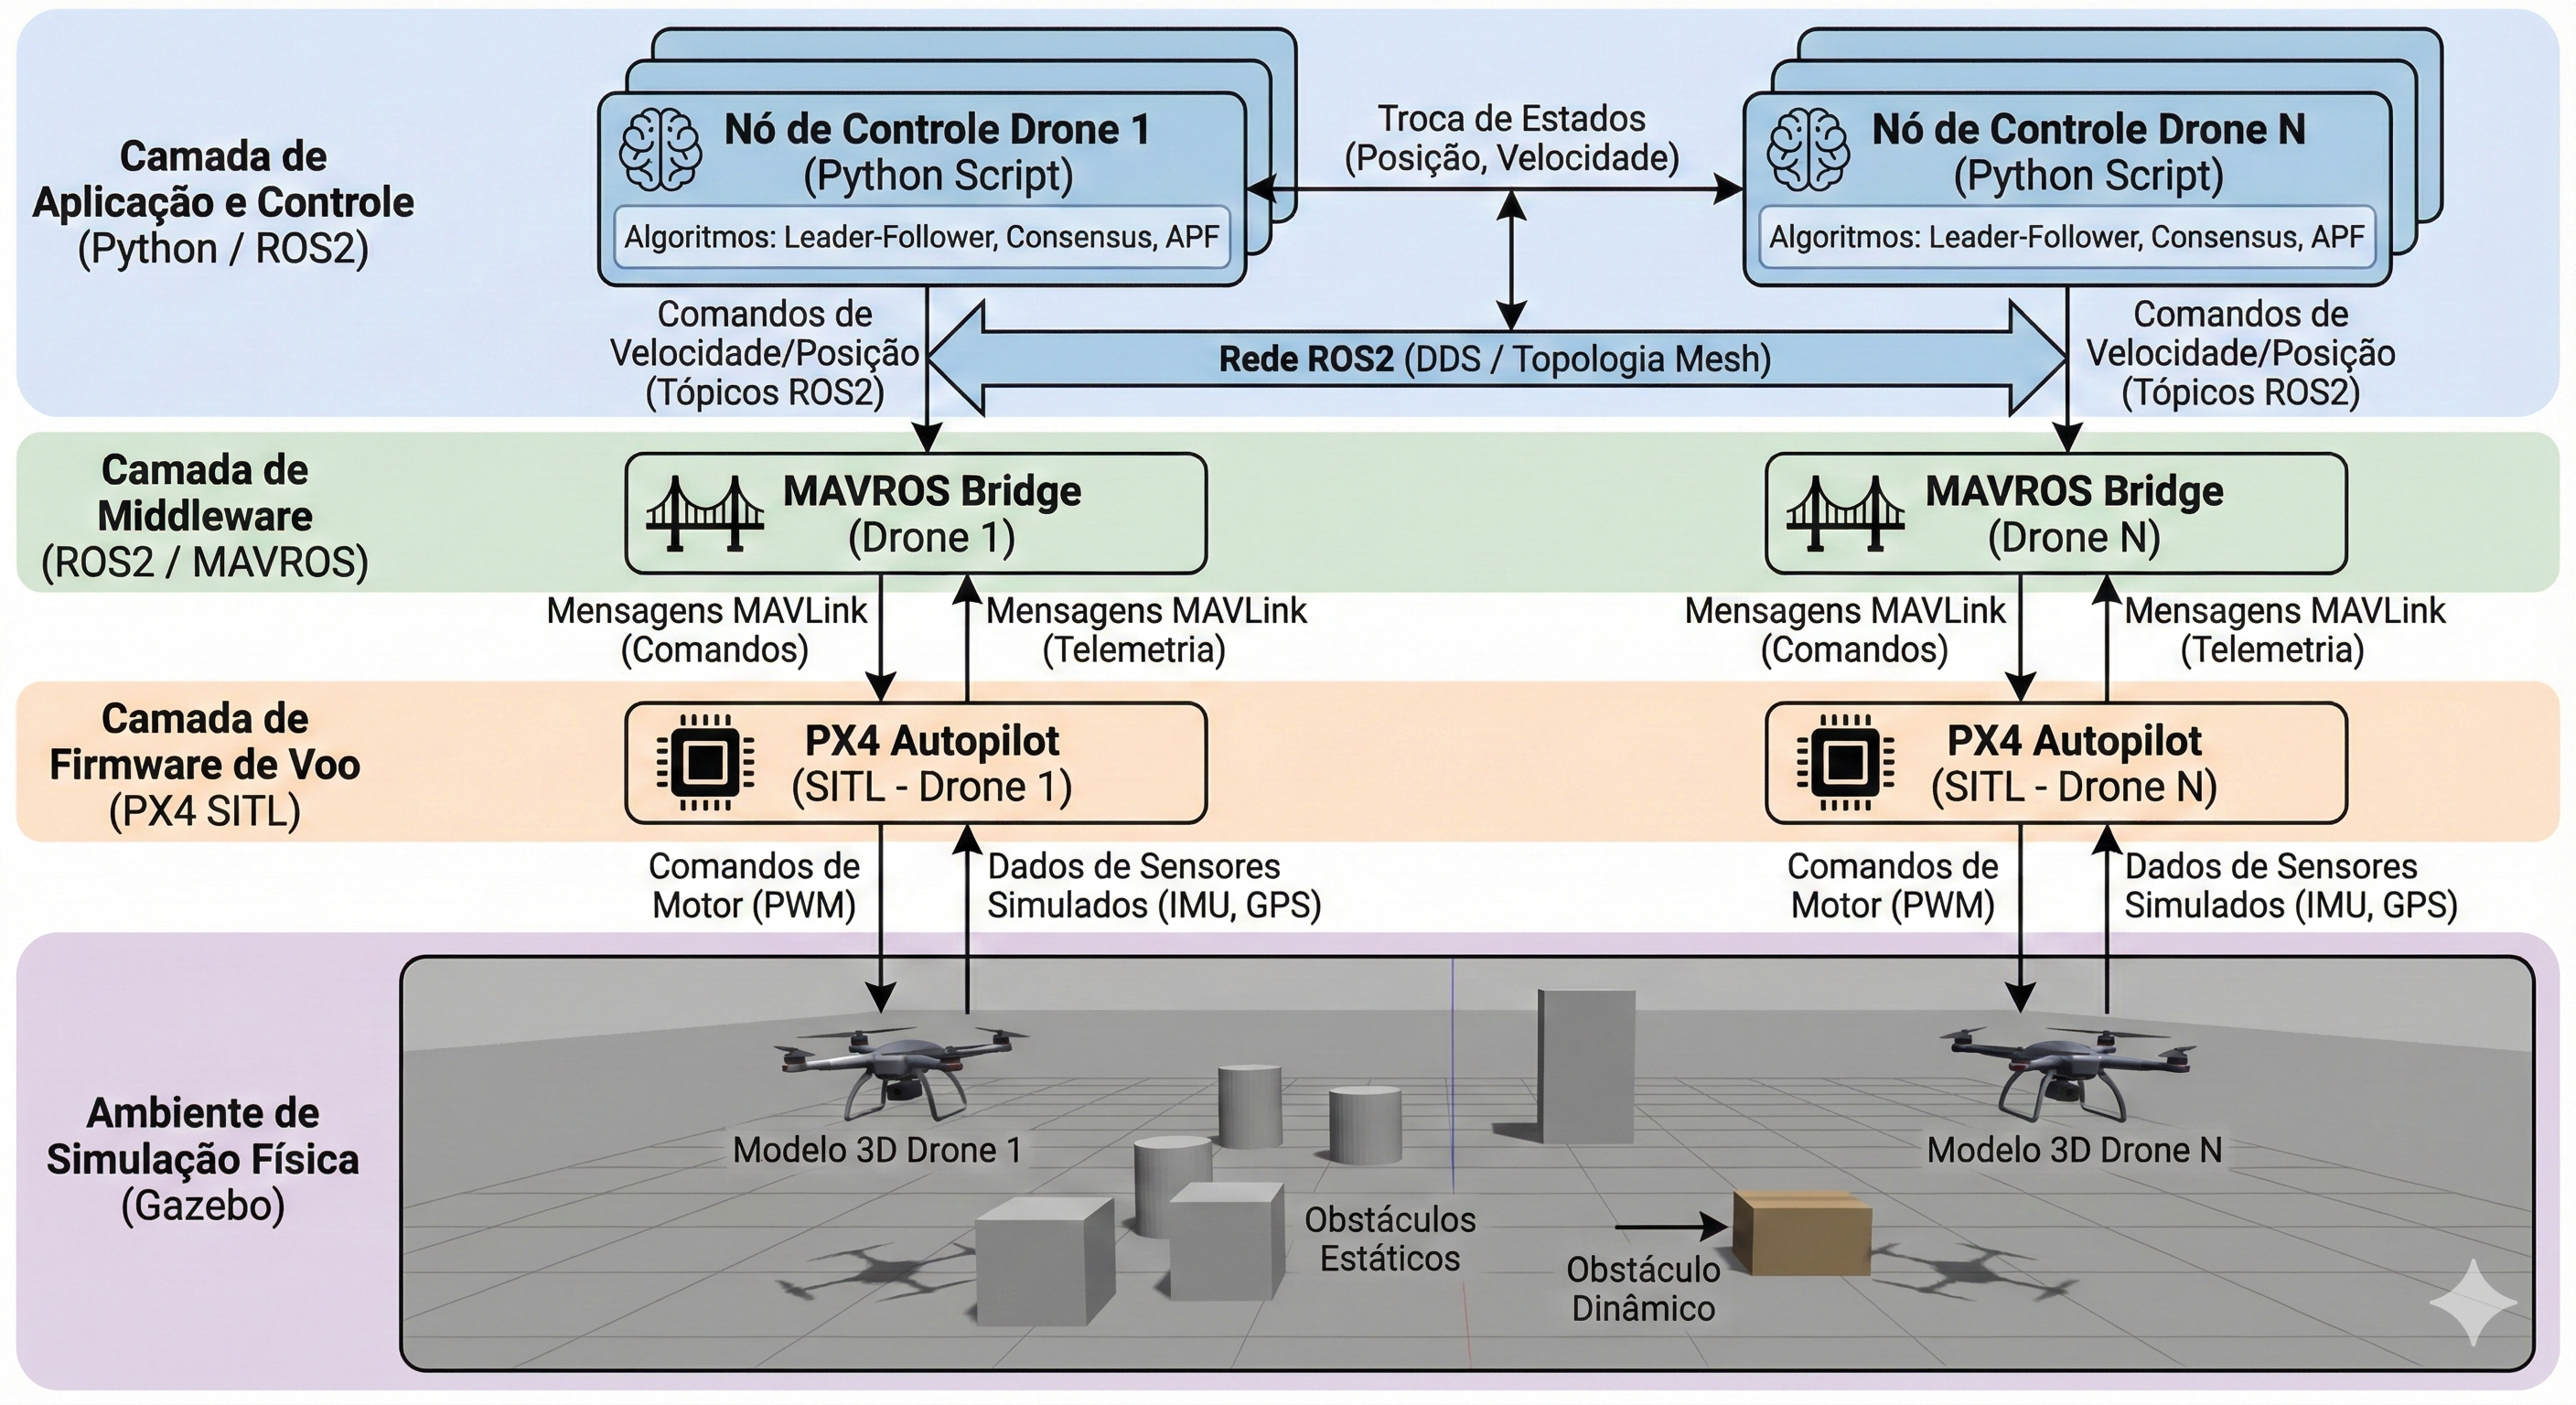
\includegraphics[width=1.0\textwidth]{images/Arquitetura1.png}
    \caption{Arquitetura do sistema de simulação proposto, integrando ROS2, MAVROS, PX4 SITL e Gazebo.}
    \label{fig:Arquitetura de simulação}
\end{figure*}

Visando abranger situações diferentes e assim conseguir avaliar os algoritmos por completo, três cenários experimentais serão configurados:

\begin{enumerate}
    \item \textbf{Espaço Livre}: ambiente sem obstáculos, destinado à análise de formação e manutenção estrutural;
    \item \textbf{Com Obstáculos Estáticos}: inserção de barreiras fixas para avaliar reconfiguração da formação;
    \item \textbf{Com Obstáculos Dinâmicos}: inclusão de obstáculos móveis, permitindo avaliar capacidade de adaptação e resposta.
\end{enumerate}

Para assegurar robustez estatística, cada experimento será repetido 10-20 vezes para cada algoritmo e cada cenário, utilizando condições iniciais distintas geradas por diferentes sementes aleatórias. Esse número de repetições foi definido com base em análise de poder estatístico, garantindo confiabilidade nas comparações entre estratégias. Cada simulação utilizará 4 drones, número suficiente para avaliar o comportamento do algoritmo no cenário.

As métricas utilizadas na avaliação serão inicialmente apenas essas:

\begin{itemize}
    \item \textbf{Erro de Formação (EF)}: distância média entre a posição real e a posição desejada de cada agente;
    \item \textbf{Tempo de Convergência (TC)}: tempo necessário para o sistema estabilizar a formação;
    \item \textbf{Estabilidade e Robustez (ER)}: capacidade de manter a formação diante de falhas de comunicação, distúrbios externos ou eventos inesperados.
\end{itemize}

Essas métricas são suficientes para avaliar a adequação do algoritmo com o cenário experimental avaliado. Os resultados serão analisados de forma quantitativa e gráfica, utilizando curvas de convergência, gráficos de dispersão e estatísticas descritivas como média, variância e desvio padrão. Essa abordagem permite comparar o desempenho das diferentes técnicas de forma detalhada e imparcial, identificando quais algoritmos — ou combinações — apresentam maior eficácia em cada tipo de cenário.

Por fim, o conjunto de procedimentos adotados e a arquitetura de simulação proposta garantem reprodutibilidade, comparabilidade e rigor experimental, permitindo que esta pesquisa contribua de maneira sólida para o avanço do estudo de controle em enxames de VANTs.




\section{Cronograma}

De acordo com a metodologia proposta, o cronograma apresentado na Tabela~\ref{tab:cronograma} organiza as etapas previstas para os próximos cinco meses, distribuindo as atividades de forma sequencial e alinhada aos objetivos do trabalho.

\begin{table*}[!ht]
\centering
\small % reduz o tamanho da fonte para caber na página
\caption{Cronograma de atividades ao longo de cinco meses.}
\label{tab:cronograma}
\renewcommand{\arraystretch}{1.2}
\begin{tabular}{|p{6.5cm}|c|c|c|c|c|}
\hline
\textbf{Atividade} & \textbf{Fevereiro} & \textbf{Março} & \textbf{Abril} & \textbf{Maio}  & \textbf{Junho} \\ \hline

Revisão dos algoritmos e requisitos             & x & x &   &   &   \\ \hline
Implementação dos algoritmos simples (Python)   & x & x &   &   &   \\ \hline
Comparação visual e ajustes                     & x & x &   &   &   \\ \hline
Configuração ROS2, Gazebo e PX4 SITL            & x & x &   &   &   \\ \hline
Cenário 1 (livre)                               &   &   & x &   &   \\ \hline
Cenário 2 (obstáculos estáticos)                &   &   & x &   &   \\ \hline
Cenário 3 (obstáculos dinâmicos)                &   &   & x &   &   \\ \hline
Execuções (10--20 simulações por cenário)       &   &   & x & x &   \\ \hline
Validação dos dados e reexecuções               &   &   &   & x &   \\ \hline
Cálculo das métricas e gráficos                 &   &   &   & x &   \\ \hline
Análise comparativa e conclusões                &   &   &   & x & x \\ \hline
Redação (resultados, conclusão, discussão)      &   &   &   & x & x \\ \hline
Revisão final e preparação da defesa            &   &   &   &   & x \\ \hline

\end{tabular}
\end{table*}


% \begin{declarations}

% \begin{acknowledgements}
% ESTA DECLARAÇÃO É OPCIONAL. Este é um texto de agradecimentos com várias linhas. Lorem ipsum dolor sit amet, consectetur adipiscing elit, sed do eiusmod tempor incididunt ut labore et dolore magna aliqua. Ut enim ad minim veniam, quis nostrud exercitation ullamco laboris nisi ut aliquip ex ea commodo consequat.
% \end{acknowledgements}


% \begin{funding}
% ESTA DECLARAÇÃO É OPCIONAL. Esta pesquisa foi financiada por lorem ipsum dolor sit amet, consectetur adipiscing elit.
% \end{funding}

% \begin{contributions}
% ESTA DECLARAÇÃO É OBRIGATÓRIA. 
% \textit{Considerar o Código de Conduta da SBC.
% Participação em autoria: espera-se que todos os autores de um trabalho publicado 
% ou submetido para publicação, tenham tido efetiva participação no respectivo trabalho.}
% Sugerimos que os autores descrevam sua contribuição usando 
% a Taxonomia CRediT (\href{https://credit.niso.org/}{https://credit.niso.org/}) como neste exemplo: 
% JV contribuiu para a concepção deste estudo. CB, RP e CM realizaram os experimentos. 
% JV é o principal contribuidor e escritor deste manuscrito. 
% Todos os autores leram e aprovaram o manuscrito final. 
% \end{contributions}

% \begin{interests}
% ESTA DECLARAÇÃO É OBRIGATÓRIA. 
% Se não houver conflitos de interesse, os autores devem declarar: 
% ``Os autores declaram que não têm nenhum conflito de interesses''. 
% Caso contrário, a declaração deve ser: 
% ``Os autores declaram que têm os seguintes conflitos de interesses: 
% lorem ipsum dolor sit amet, consectetur adipiscing elit.''
% \end{interests}

% \begin{materials}
% ESTA DECLARAÇÃO É OBRIGATÓRIA. 
% \textit{Considerar o Código de Conduta da SBC. 
% Reprodutibilidade de resultados de pesquisa: 
% nos casos pertinentes, recomenda-se que artigos indiquem 
% a disponibilidade pública de material utilizado nas revisões, 
% de modo a facilitar a reprodução dos respectivos resultados por outros pesquisadores.}
% %
% Se os autores disponibilizaram seus dados e/ou códigos abertamente, a declaração deve ser: 
% ``Os dados e outros materiais criados e/ou usados nesta revisão da literatura
% estão disponíveis em \ldots''. 
% Caso contrário, a declaração deve ser: 
% ``Os dados e outros materiais criados e/ou usados nesta revisão da literatura 
% serão disponibilizados mediante solicitação''. 
% %
% Todo o material suplementar disponibilizado publicamente pelos autores aparecerá 
% na página de publicação do artigo em caso de aceitação. 
% \end{materials}

% \begin{aitools}
% ESTA DECLARAÇÃO É OBRIGATÓRIA.  
% \textit{Considerar o Código de Conduta da SBC.
% Uso de Inteligência Artificial (IA) Generativa: 
% a utilização de ferramentas e tecnologias de IA Generativa para geração de conteúdos, 
% na escrita e/ou revisão do conteúdo de artigos, deve ser declarada explicitamente no trabalho.} 
% A declaração deve ocorrer nesta seção, definida especificamente para este fim.
% Deve-se listar as ferramentas (e suas versões) e descrever onde foram empregadas, por exemplo, 
% textos, tabelas, gráficos, citações, etc. 
% Essas ferramentas \textbf{não} podem ser listadas como autores de um artigo. 
% O uso de tais ferramentas não exime os autores da responsabilidade 
% sobre todo o seu conteúdo, inclusive no caso de ser identificado plágio.
% %
% Se os autores não utilizaram tais ferramentas, a declaração deve ser: 
% ``Os autores não utilizaram ferramentas de IA generativa no desenvolvimento do estudo''.
% %
% \end{aitools}

% \begin{furtherinformation}
% Manuscritos devem indicar explicitamente como as questões éticas da pesquisa foram abordadas e gerenciadas, 
% incluindo a aprovação da pesquisa por um comitê de ética, quando aplicável.
% \end{furtherinformation}

% \end{declarations}


\section{Resultados}
\label{sec:resultados}

Esta seção apresenta e analisa os resultados obtidos nas simulações dos algoritmos de controle de formação implementados. As execuções foram realizadas no simulador Gazebo, integrado ao PX4 SITL e ao ROS~2, com um enxame de 8 drones. Para cada algoritmo foram registradas as seguintes métricas: tempo total de convergência da missão, custo computacional (tempo médio e pico de cálculo por iteração, uso de CPU e consumo de RAM), distância média percorrida pelo enxame e margem mínima de segurança mantida em relação a obstáculos.

Os cenários de simulação foram organizados em quatro configurações, representadas pelas subpastas \texttt{1}, \texttt{2}, \texttt{3} e \texttt{4} dentro de cada algoritmo:

\begin{itemize}
    \item \textbf{Cenário 1}: mundo com obstáculos estáticos, sem vento;
    \item \textbf{Cenário 2}: mundo com obstáculos estáticos, com vento;
    \item \textbf{Cenário 3}: mundo livre (sem obstáculos), sem vento;
    \item \textbf{Cenário 4}: mundo livre (sem obstáculos), com vento.
\end{itemize}

É importante observar que nem todos os algoritmos foram executados em todos os cenários. Os algoritmos \textit{Behavior-Based}, \textit{Consensus-Based} e \textit{Leader-Follower} não possuem mecanismo de desvio de obstáculos, de modo que suas execuções ficaram restritas aos cenários 3 e 4. O algoritmo híbrido \textit{Virtual Structure + APF} (\textit{Switching VS-APF}), por sua vez, foi projetado especificamente para operar em ambientes com obstáculos e foi avaliado nos cenários 1 e 2.

\subsection{Cobertura dos Experimentos por Cenário}

A Tabela~\ref{tab:cobertura} resume os cenários em que cada algoritmo foi executado com sucesso, indicando também a causa das ausências.

\begin{table}[ht]
\centering
\caption{Cobertura dos algoritmos por cenário de simulação.}
\label{tab:cobertura}
\footnotesize % Reduz levemente o tamanho da fonte
\setlength{\tabcolsep}{4pt} % Reduz o espaço em branco entre as colunas
\begin{tabular}{|l|c|c|c|c|}
\hline
\textbf{Algoritmo} & \textbf{Cen. 1} & \textbf{Cen. 2} & \textbf{Cen. 3} & \textbf{Cen. 4} \\ \hline
APF & \checkmark & \checkmark & \checkmark & \checkmark \\ \hline
Behavior-Based & -- & -- & \checkmark & \checkmark \\ \hline
Consensus-Based & -- & -- & \checkmark & \checkmark \\ \hline
Leader-Follower & -- & -- & \checkmark & \checkmark \\ \hline
Virtual Structure & -- & -- & \checkmark & \checkmark \\ \hline
Híbrido VS-APF & \checkmark & \checkmark & -- & -- \\ \hline
\end{tabular}
\end{table}

Os traços (``--'') nos cenários com obstáculos para os algoritmos \textit{Behavior-Based}, \textit{Consensus-Based}, \textit{Leader-Follower} e \textit{Virtual Structure} decorrem da incapacidade desses métodos de tratar colisões: sem um mecanismo de repulsão ativo, os drones não conseguem contornar os obstáculos e a missão não converge. Nos cenários livres, o \textit{Híbrido VS-APF} não foi avaliado pois sua motivação principal é, precisamente, a navegação em ambientes obstruídos.

\subsection{Tempo de Convergência da Missão}

O tempo de convergência representa o intervalo entre a decolagem e o pouso completo de todos os drones no ponto-alvo. Os resultados consolidados são apresentados na Tabela~\ref{tab:tempo}.

\begin{table}[ht]
\centering
\caption{Tempo total de convergência da missão por algoritmo e cenário.}
\label{tab:tempo}
\footnotesize % Reduz levemente o tamanho da fonte
\setlength{\tabcolsep}{4pt} % Reduz o espaço em branco entre as colunas
\begin{tabular}{|l|c|c|c|c|}
\hline
\textbf{Algoritmo} & \textbf{Cen. 1 (s)} & \textbf{Cen. 2 (s)} & \textbf{Cen. 3 (s)} & \textbf{Cen. 4 (s)} \\ \hline
APF & 190,71 & 170,82 & 148,42 & 165,53 \\ \hline
Behavior-Based & -- & -- & 150,49 & 146,82 \\ \hline
Consensus-Based & -- & -- & 104,13 & 104,13 \\ \hline
Leader-Follower & -- & -- & 162,39 & 159,89 \\ \hline
Virtual Structure & -- & -- & 34,98 & 37,98 \\ \hline
Híbrido VS-APF & 121,46 & 121,62 & -- & -- \\ \hline
\end{tabular}
\end{table}

O \textit{Virtual Structure} apresentou o menor tempo de convergência dentre todos os algoritmos avaliados nos cenários livres, completando a missão em aproximadamente 35--38 segundos. Esse resultado é explicado pela natureza do algoritmo: ao tratar o enxame como um corpo rígido com posições absolutas predefinidas, os drones seguem uma trajetória sincronizada e determinística sem necessidade de negociação iterativa. Esse ganho de velocidade, porém, implica rigidez estrutural e ausência de capacidade de desvio autônomo, o que inviabiliza seu uso em ambientes com obstáculos.

O \textit{Consensus-Based} obteve o segundo melhor tempo nos cenários livres (104 segundos em ambos), com notável estabilidade: o resultado foi idêntico nos cenários 3 e 4, sugerindo que a adição de vento não afetou significativamente a dinâmica de convergência distribuída do método. Já o \textit{Leader-Follower} completou a missão em cerca de 161 segundos, com pequena variação entre os dois cenários livres.

O \textit{APF} apresentou os maiores tempos de convergência em todos os cenários, atingindo 190,71 segundos no cenário 1. O custo de recalcular continuamente campos de potencial para múltiplos pares drone-obstáculo a cada iteração introduz um atraso no controle que se acumula ao longo da missão. O \textit{Híbrido VS-APF}, por sua vez, reduziu esse tempo para aproximadamente 121 segundos nos cenários com obstáculos, uma melhoria de cerca de 37\% em relação ao APF puro no cenário 1.

\subsection{Custo Computacional}

A Tabela~\ref{tab:custo} apresenta as métricas de custo computacional registradas para cada algoritmo: tempo médio de cálculo por iteração do \textit{loop} de controle, pico máximo de cálculo (gargalo), uso médio de CPU e consumo de RAM.

\begin{table*}[ht]
\centering
\caption{Métricas de custo computacional por algoritmo e cenário.}
\label{tab:custo}
\renewcommand{\arraystretch}{1.15}
\begin{tabular}{|p{3.2cm}|c|c|c|c|c|}
\hline
\textbf{Algoritmo} & \textbf{Cenário} & \textbf{Méd. cálculo (ms)} & \textbf{Pico (ms)} & \textbf{CPU (\%)} & \textbf{RAM (MB)} \\ \hline
APF             & 1 & 3,33 & 17,46 & 2,10 & 52,73 \\ \hline
APF             & 2 & 3,74 & 20,88 & 2,00 & 52,46 \\ \hline
APF             & 3 & 2,79 & 13,39 & 1,74 & 52,55 \\ \hline
APF             & 4 & 3,70 & 19,03 & 2,00 & 52,49 \\ \hline
Behavior-Based  & 3 & 0,76 & 2,92  & 1,00 & 52,16 \\ \hline
Behavior-Based  & 4 & 0,79 & 4,14  & 1,03 & 52,24 \\ \hline
Consensus-Based & 3 & 0,38 & 1,61  & 1,73 & 52,29 \\ \hline
Consensus-Based & 4 & 0,40 & 1,73  & 1,52 & 52,17 \\ \hline
Leader-Follower & 3 & 0,20 & 0,85  & 1,79 & 52,61 \\ \hline
Leader-Follower & 4 & 0,21 & 1,71  & 1,62 & 52,62 \\ \hline
Virtual Structure & 3 & 0,06 & 0,18 & 1,71 & 51,89 \\ \hline
Virtual Structure & 4 & 0,07 & 0,21 & 1,65 & 51,94 \\ \hline
Híbrido VS-APF  & 1 & 0,76 & 3,99  & 1,93 & 52,52 \\ \hline
Híbrido VS-APF  & 2 & 0,76 & 4,61  & 1,68 & 52,49 \\ \hline
\end{tabular}
\end{table*}

A diferença de custo computacional entre os algoritmos é expressiva. O \textit{Virtual Structure} é o mais eficiente: opera com apenas 0,06--0,07 ms por iteração e pico máximo de 0,18--0,21 ms, pois realiza exclusivamente operações matriciais de posição relativa com complexidade constante. O \textit{Leader-Follower} ocupa a segunda posição, com média de 0,20 ms. Esse resultado é igualmente esperado, já que o controlador proporcional-derivativo (PD) de cada seguidor envolve operações algébricas simples.

O \textit{Consensus-Based} e o \textit{Behavior-Based} operam em faixas intermediárias (0,38--0,40 ms e 0,76--0,79 ms, respectivamente). Ambos exigem iterações sobre o conjunto de vizinhos para calcular forças de coesão, alinhamento e separação ou atualizar o vetor de consenso, o que eleva moderadamente o custo por loop.

O \textit{APF} é o algoritmo mais custoso, com média de 2,79--3,74 ms e picos de até 20,88 ms (cenário 2). Esse comportamento decorre do cálculo iterativo dos campos de potencial para todos os pares drone-obstáculo e drone-drone a cada ciclo de controle, cuja complexidade cresce com o número de agentes e com a densidade de obstáculos no ambiente. O pico de gargalo no cenário 2 (obstáculos com vento) é superior ao do cenário 1, evidenciando que a perturbação do vento força renegociações mais frequentes dos campos de força.

O \textit{Híbrido VS-APF} alcança um equilíbrio notável: com média de 0,76 ms, é aproximadamente quatro a cinco vezes mais rápido por iteração que o APF puro, mesmo operando em ambientes com obstáculos. Isso ocorre porque, durante os trechos sem obstáculos próximos, o modo \textit{Virtual Structure} (muito mais leve) está ativo; o APF só é ativado pontualmente, quando algum drone entra na zona de influência de um obstáculo.

Quanto ao consumo de RAM, todos os algoritmos permanecem em uma faixa estreita de 51,89--52,73 MB, indicando que nenhum deles impõe demandas significativas de memória para enxames de 8 drones.

\subsection{Distância Percorrida pelo Enxame}

A distância média percorrida pelos drones durante a missão é um indicador complementar à análise de convergência, pois revela a eficiência das trajetórias geradas por cada algoritmo. Os valores são apresentados na Tabela~\ref{tab:distancia}.

\begin{table}[ht]
\centering
\caption{Distância média percorrida pelo enxame por algoritmo e cenário.}
\label{tab:distancia}
\begin{tabular}{|p{3.2cm}|c|c|}
\hline
\textbf{Algoritmo} & \textbf{Cenário} & \textbf{Dist. média (m)} \\ \hline
APF             & 1 & 62,76 \\ \hline
APF             & 2 & 59,24 \\ \hline
APF             & 3 & 50,89 \\ \hline
APF             & 4 & 60,82 \\ \hline
Behavior-Based  & 3 & 53,72 \\ \hline
Behavior-Based  & 4 & 54,27 \\ \hline
Consensus-Based & 3 & 35,84 \\ \hline
Consensus-Based & 4 & 38,02 \\ \hline
Leader-Follower & 3 & 64,34 \\ \hline
Leader-Follower & 4 & 65,10 \\ \hline
Virtual Structure & 3 & 78,69 \\ \hline
Virtual Structure & 4 & 78,77 \\ \hline
Híbrido VS-APF  & 1 & 91,86 \\ \hline
Híbrido VS-APF  & 2 & 90,79 \\ \hline
\end{tabular}
\end{table}

O \textit{Consensus-Based} gerou as trajetórias mais curtas (35,84--38,02 m), uma consequência direta do mecanismo de convergência por consenso: ao buscar um ponto médio coletivo iterativamente, os drones tendem a se aproximar uns dos outros antes de avançar em direção ao objetivo, encurtando as trajetórias individuais. O \textit{Híbrido VS-APF} registrou as maiores distâncias (90--92 m), pois os desvios ativos em torno dos obstáculos, momento em que o modo APF está ativo, geram percursos mais longos do que uma rota direta.

O \textit{Virtual Structure} apresenta distâncias uniformes e elevadas (78,69--78,77 m) com variação praticamente nula entre os drones, reflexo da rigidez do corpo virtual: todos percorrem a mesma trajetória geométrica, diferenciando-se apenas pelo offset de posição relativa.

\subsection{Segurança em Relação a Obstáculos}

A margem de segurança mínima, definida como a menor distância registrada entre cada drone e qualquer obstáculo ao longo da missão, é a métrica mais crítica para avaliar a aptidão de cada algoritmo em ambientes obstruídos. A Tabela~\ref{tab:seguranca} apresenta os valores por drone nos cenários relevantes.

\begin{table*}[ht]
\centering
\caption{Margem mínima de segurança (em metros) em relação a obstáculos, por drone e cenário. ``--'' indica cenários sem obstáculos.}
\label{tab:seguranca}
\renewcommand{\arraystretch}{1.1}
\begin{tabular}{|p{3.0cm}|c|c|c|c|c|c|c|c|c|}
\hline
\textbf{Algoritmo (cen.)} & \textbf{D0} & \textbf{D1} & \textbf{D2} & \textbf{D3} & \textbf{D4} & \textbf{D5} & \textbf{D6} & \textbf{D7} & \textbf{Mín. geral} \\ \hline
APF (1)          & 1,98 & 2,09 & 2,06 & 2,12 & 2,06 & 1,95 & 1,94 & 2,05 & 1,94 \\ \hline
APF (2)          & 2,07 & 2,00 & 1,99 & 2,11 & 2,14 & 1,83 & 2,03 & 1,88 & 1,83 \\ \hline
Híbrido VS-APF (1) & 2,10 & 2,09 & 2,12 & 2,07 & 2,11 & 2,05 & 2,15 & 2,49 & 2,05 \\ \hline
Híbrido VS-APF (2) & 2,12 & 2,01 & 2,06 & 2,07 & 2,12 & 2,11 & 2,08 & 2,48 & 2,01 \\ \hline
\end{tabular}
\end{table*}

Tanto o \textit{APF} quanto o \textit{Híbrido VS-APF} mantiveram margens de segurança consistentes e superiores a 1,8 m em todos os drones e cenários testados. O \textit{Híbrido VS-APF} apresentou margens ligeiramente mais uniformes entre os drones, com valores entre 2,01 m e 2,49 m, sugerindo que a alternância entre os modos \textit{Virtual Structure} e \textit{APF} distribui melhor o espaçamento relativo ao enxame inteiro.

Os algoritmos que operam apenas em ambientes livres (Behavior-Based, Consensus-Based, Leader-Follower e Virtual Structure) retornam margem ``\textit{inf}'' (infinita) nesses cenários, pois o ambiente não contém obstáculos. Quando expostos a ambientes com obstáculos, esses algoritmos não possuem mecanismo de desvio e, portanto, não convergem — o que justifica a exclusão dessas configurações dos experimentos, conforme discutido na Seção~\ref{sec:resultados}.

\subsection{Análise Comparativa Geral}

A Tabela~\ref{tab:comparativo} consolida as principais métricas médias por algoritmo, facilitando a comparação direta entre as abordagens.

\begin{table*}[ht]
\centering
\caption{Comparativo geral das métricas médias por algoritmo (cenários em que houve execução completa).}
\label{tab:comparativo}
\renewcommand{\arraystretch}{1.15}
\resizebox{\textwidth}{!}{%
\begin{tabular}{|l|c|c|c|c|c|}
\hline
\textbf{Algoritmo} & \textbf{Tempo médio (s)} & \textbf{Cálculo médio (ms)} & \textbf{Pico médio (ms)} & \textbf{Dist. média (m)} & \textbf{Seg. mín. (m)} \\ \hline
APF                & 168,87 & 3,39 & 17,69 & 58,43 & 1,83 \\ \hline
Behavior-Based     & 148,66 & 0,78 &  3,53 & 53,99 & --   \\ \hline
Consensus-Based    & 104,13 & 0,39 &  1,67 & 36,93 & --   \\ \hline
Leader-Follower    & 161,14 & 0,20 &  1,28 & 64,72 & --   \\ \hline
Virtual Structure  &  36,48 & 0,06 &  0,20 & 78,73 & --   \\ \hline
Híbrido VS-APF     & 121,54 & 0,76 &  4,30 & 91,33 & 2,01 \\ \hline
\end{tabular}%
}
\end{table*}

A análise integrada revela três perfis distintos de desempenho:

\textbf{Alta eficiência computacional, cenários livres.} O \textit{Virtual Structure} e o \textit{Leader-Follower} destacam-se pelo baixíssimo custo de cálculo (0,06--0,20 ms/loop) e por tempos de convergência extremamente baixos no caso do \textit{Virtual Structure} (36 s). Contudo, a ausência de qualquer mecanismo reativo limita sua aplicabilidade a missões em espaços abertos e previamente mapeados. O \textit{Virtual Structure}, em particular, impõe trajetórias idênticas a todos os drones, o que pode ser vantajoso em formações de precisão mas constitui uma restrição severa em ambientes dinâmicos.

\textbf{Equilíbrio entre escalabilidade e robustez distribuída.} O \textit{Consensus-Based} e o \textit{Behavior-Based} operam de forma totalmente distribuída, com custo computacional moderado e boa robustez a perturbações como vento — evidenciada pela estabilidade do tempo de convergência do \textit{Consensus-Based} nos cenários 3 e 4. Esses métodos são os mais indicados para enxames grandes em ambientes sem obstáculos estruturais, onde a emergência coletiva é suficiente para guiar o grupo.

\textbf{Aptidão para ambientes obstruídos.} O \textit{APF} e o \textit{Híbrido VS-APF} são os únicos algoritmos capazes de operar com segurança em ambientes com obstáculos. O \textit{Híbrido VS-APF} demonstrou vantagem significativa sobre o \textit{APF} puro em dois aspectos: reduziu o tempo de missão em aproximadamente 37\% (de 180 s para 121 s nos cenários com obstáculos) e operou com custo computacional quatro vezes menor por iteração (0,76 ms versus 3,39 ms em média), mantendo margens de segurança equivalentes ou superiores. Esses resultados validam a hipótese de hibridização proposta neste trabalho: a comutação entre o modo \textit{Virtual Structure} (ativado em trechos livres) e o modo \textit{APF} (ativado somente na proximidade de obstáculos) permite reunir a eficiência computacional do primeiro com a capacidade reativa do segundo.


\section{Conclusão e Trabalhos Futuros}
\label{sec:conclusao}

Este trabalho apresentou uma análise abrangente e comparativa de algoritmos de controle cooperativo para enxames de VANTs, abordando desde a fundamentação teórica de sistemas multiagente até a validação empírica em um ambiente de simulação de alta fidelidade (Gazebo, PX4 SITL e ROS~2). O foco principal residiu em compreender como diferentes estratégias lidam com o compromisso (\textit{trade-off}) entre a manutenção rigorosa de formações geométricas, a evasão de obstáculos e o custo computacional embarcado.

Os experimentos realizados em cenários livres de obstáculos (Mundos 3 e 4) evidenciaram a superioridade computacional de abordagens fundamentadas rigidamente na geometria ou hierarquia, como o \textit{Virtual Structure} e o \textit{Leader-Follower}. Estas técnicas garantiram convergência rápida e estabilidade estrutural impecável com um esforço de processamento quase nulo para as CPUs dos agentes. Contudo, ao submeter essas mesmas estratégias a ambientes complexos com obstáculos estáticos (Mundos 1 e 2), ficou provado que a rigidez geométrica desses algoritmos os torna vulneráveis, culminando em falhas operacionais por ausência de um mecanismo reativo de repulsão.

Por outro lado, o uso exclusivo de Campos Potenciais Artificiais (\textit{APF}) conferiu ao enxame total segurança contra colisões em ambientes densos. No entanto, as métricas extraídas revelaram que essa segurança tem um custo elevado: o APF puro gerou os maiores tempos de processamento médio e os maiores picos de gargalo computacional. Além disso, ao tentar equilibrar simultaneamente forças conflitantes de atração global e repulsão local, o algoritmo alongou significativamente o tempo total da missão.

A principal contribuição consolidada por estas análises foi a validação prática do modelo de Chaveamento de Modos (\textit{Switching VS $\rightarrow$ APF $\rightarrow$ VS}). Ao operar primariamente sob a lógica de baixo custo do \textit{Virtual Structure} e delegar a evasão ao \textit{APF} apenas em zonas críticas de colisão, o sistema híbrido alcançou o cenário ótimo de operação: preservou a integridade física dos veículos e reduziu de forma substancial o tempo médio de processamento por iteração (cerca de quatro vezes menor em comparação ao APF puro). Ademais, a estratégia híbrida mitigou o fenômeno de mínimos locais, encurtando o tempo total de missão nos cenários com obstáculos em quase 37\% frente à abordagem puramente reativa.

A pesquisa também evidenciou o impacto das condições atmosféricas dinâmicas. A introdução de vento nos simuladores amplificou os picos de processamento de todos os algoritmos, exigindo recálculos mais frequentes das malhas de controle para corrigir derivas inerciais. Esse achado destaca a importância crítica de se adotar arquiteturas de controle que possuam ampla folga computacional (\textit{overhead} reduzido) na CPU embarcada.

Como trabalhos futuros, sugere-se:
\begin{itemize}
    \item A transição dos algoritmos avaliados para plataformas de hardware real (\textit{Hardware-In-The-Loop} e voos \textit{outdoor}), com o intuito de mensurar o impacto da degradação real do sinal de comunicação (latência e ruído) no comportamento dos agentes distribuídos;
    \item A introdução de obstáculos dinâmicos no ambiente de simulação, visando avaliar o tempo de resposta da malha de chaveamento híbrido frente a ameaças com trajetórias não previsíveis;
    \item A incorporação de lógicas de tolerância a falhas na abordagem \textit{Leader-Follower}, implementando a eleição descentralizada de um novo VANT líder em caso de perda de comunicação ou inoperância do agente principal.
\end{itemize}

Em suma, este estudo propõe um \textit{framework} estruturado de avaliação e fornece diretrizes sólidas para o design e a otimização de enxames de VANTs. Os resultados comprovam que arquiteturas de controle híbridas e baseadas em chaveamento de estados representam o caminho mais promissor, seguro e eficiente para a execução de missões cooperativas e autônomas no mundo real.


\bibliographystyle{apalike-sol}
\bibliography{refs}

\end{document}
